%% Based on a TeXnicCenter-Template by Tino Weinkauf.
%%%%%%%%%%%%%%%%%%%%%%%%%%%%%%%%%%%%%%%%%%%%%%%%%%%%%%%%%%%%%

%%%%%%%%%%%%%%%%%%%%%%%%%%%%%%%%%%%%%%%%%%%%%%%%%%%%%%%%%%%%%
%% HEADER
%%%%%%%%%%%%%%%%%%%%%%%%%%%%%%%%%%%%%%%%%%%%%%%%%%%%%%%%%%%%%
\documentclass[12pt]{report}
% Alternative Options:
%	Paper Size: a4paper / a5paper / b5paper / letterpaper / legalpaper / executivepaper
% Duplex: oneside / twoside
% Base Font Size: 10pt / 11pt / 12pt
\setlength{\parskip}{1em}

%% Packages for Graphics & Figures %%%%%%%%%%%%%%%%%%%%%%%%%%
\usepackage{graphicx} %%For loading graphic files
%\usepackage{subfig} %%Subfigures inside a figure
%\usepackage{pst-all} %%PSTricks - not useable with pdfLaTeX


%% Math Packages %%%%%%%%%%%%%%%%%%%%%%%%%%%%%%%%%%%%%%%%%%%%
\usepackage{amsmath}
\usepackage{amsthm}
\usepackage{amsfonts}
\usepackage{caption}
\usepackage{subcaption}
\newtheorem{theorem}{Theorem}


%% Line Spacing %%%%%%%%%%%%%%%%%%%%%%%%%%%%%%%%%%%%%%%%%%%%%
%\usepackage{setspace}
%\singlespacing        %% 1-spacing (default)
%\onehalfspacing       %% 1,5-spacing
%\doublespacing        %% 2-spacing


%% Other Packages %%%%%%%%%%%%%%%%%%%%%%%%%%%%%%%%%%%%%%%%%%%
%\usepackage{a4wide} %%Smaller margins = more text per page.
%\usepackage{fancyhdr} %%Fancy headings
%\usepackage{longtable} %%For tables, that exceed one page


%%%%%%%%%%%%%%%%%%%%%%%%%%%%%%%%%%%%%%%%%%%%%%%%%%%%%%%%%%%%%
%% Remarks
%%%%%%%%%%%%%%%%%%%%%%%%%%%%%%%%%%%%%%%%%%%%%%%%%%%%%%%%%%%%%
%
% TODO:
% 1. Edit the used packages and their options (see above).
% 2. If you want, add a BibTeX-File to the project
%    (e.g., 'literature.bib').
% 3. Happy TeXing!
%
%%%%%%%%%%%%%%%%%%%%%%%%%%%%%%%%%%%%%%%%%%%%%%%%%%%%%%%%%%%%%

%%%%%%%%%%%%%%%%%%%%%%%%%%%%%%%%%%%%%%%%%%%%%%%%%%%%%%%%%%%%%
%% DOCUMENT
%%%%%%%%%%%%%%%%%%%%%%%%%%%%%%%%%%%%%%%%%%%%%%%%%%%%%%%%%%%%%
\begin{document}

\pagestyle{empty} %No headings for the first pages.


%% Title Page %%%%%%%%%%%%%%%%%%%%%%%%%%%%%%%%%%%%%%%%%%%%%%%
%% ==> Write your text here or include other files.

%% The simple version:
%\title{An Overview of Semantic Segmentation and \\
			 %Pushing State of the Art}
%\author{Chase Gaudet}
%\date{} %%If commented, the current date is used.
%\maketitle

%% The nice version:
%% Based on a TeXnicCenter-Template by Tino Weinkauf.
%%%%%%%%%%%%%%%%%%%%%%%%%%%%%%%%%%%%%%%%%%%%%%%%%%%%%%%%%%%%%

%%%%%%%%%%%%%%%%%%%%%%%%%%%%%%%%%%%%%%%%%%%%%%%%%%%%%%%%%%%%%
%% Deckblatt
%%%%%%%%%%%%%%%%%%%%%%%%%%%%%%%%%%%%%%%%%%%%%%%%%%%%%%%%%%%%%
%%
%% ATTENTION: You need a main file to use this one here.
%%            Use the command "\input{filename}" in your
%%            main file to include this file.
%%

\begin{titlepage}

\begin{center}

%\vspace*{1cm}
\Large
\textsc{Deep Quaternion Networks}\\

\vspace{4cm}

%\LARGE
\textsc{Prospectus\\[0.5\baselineskip]
by\\[0.5\baselineskip]
Chase Gaudet}\\

\vspace{4cm}
\textsc{\today}\\ %%Date - better you write it yourself.

\vspace{1cm}
\textsc{Supervisor:\\
Dr. Anthony Maida}\\

\vspace{1cm}
\textsc{University of Louisiana at Lafayette\\
Faculty of Computer Science}\\

\end{center}

\end{titlepage}
 %%You need a file 'titlepage.tex' for this.
%% ==> TeXnicCenter supplies a possible titlepage file
%% ==> with its templates (File | New from Template...).


%% Front Matter Section %%%%%%%%%%%%%%%%%%%%%%%%%%%%%%%%%%%%%
\chapter*{Abstract}
The field of deep learning has seen significant advancement in recent years.
However, much of the existing work has been focused on real-valued numbers.
Recent work has shown that a deep learning system using the complex numbers can be deeper for a fixed parameter budget compared to its real-valued counterpart.
In this work, we explore the benefits of generalizing one step further into the hyper-complex numbers, quaternions specifically, and provide the architecture components needed to build deep quaternion networks.
We go over quaternion convolutions, present a quaternion weight initialization scheme, and present algorithms for quaternion batch-normalization.
These pieces are tested in a classification model by end-to-end training on the CIFAR-10 and CIFAR-100 data sets and a segmentation model by end-to-end training on the KITTI Road Segmentation data set. 
The quaternion networks show improved convergence compared to real-valued and complex-valued networks, especially on the segmentation task.


\chapter*{Dedication}
PLACEHOLDER


%% Inhaltsverzeichnis %%%%%%%%%%%%%%%%%%%%%%%%%%%%%%%%%%%%%%%
\tableofcontents %Table of contents
\cleardoublepage %The first chapter should start on an odd page.

\pagestyle{plain} %Now display headings: headings / fancy / ...



%% Chapters %%%%%%%%%%%%%%%%%%%%%%%%%%%%%%%%%%%%%%%%%%%%%%%%%
%% ==> Write your text here or include other files.

%\input{intro} %You need a file 'intro.tex' for this.

\chapter{Quaternions}
The quaternions are a number system that extends the complex numbers. 
They were first described by Irish mathematician William Rowan Hamilton in 1843 and applied to mechanics in three-dimensional space. 
In modern mathematical language, quaternions form a four-dimensional associative normed division algebra over the real numbers, and therefore also a domain.
In this chapter we will define operations on the quaternion algebra, draw connection to the complex numbers and $\mathbb{R}^3$, and show some real world use cases of quaternions.


\section{Quaternion Algebra}\label{s:quatalg}
In 1833 Hamilton proposed complex numbers $\mathbb{C}$ be defined as the set $\mathbb{R}^2$ of ordered pairs $(a, b)$ of real numbers.
He then began working to see if triplets $(a,b,c)$ could extend multiplication of complex numbers.
In 1843 he discovered a way to multiply in four dimensions instead of three, but the multiplication lost commutativity.
This construction is now known as quaternions.
Quaternions are composed of four components, one real part, and three imaginary parts.
Typically denoted as
\begin{equation}
\mathbb{H} = \{a + b\textit{i} + c\textit{j} + d\textit{k}~:~a,b,c,d \in \mathbb{R}\}
\label{eq:quaternion1}
\end{equation}
where $a$ is the real part, $(i,j,k)$ denotes the three imaginary axis, and $(b,c,d)$ denotes the three imaginary components.
Sometimes $a$ is referred to as the scalar part and $(a,b,c)$ as the vector part.
Quaternions are governed by the following arithmetic:
\begin{equation}
i^2=j^2=k^2=ijk=-1
\label{eq:quarternion2}
\end{equation}
which, by enforcing distributivity, leads to the noncommutative multiplication rules
\begin{equation}
ij=k,~jk=i,~ki=j,~ji=-k,~kj=-i,~ik=-j
\label{eq:quarternion3}
\end{equation}


\subsection{Addition and Multiplication}
The addition of two quaternions acts component wise, exactly the same as two complex numbers.
Consider the quaternion $q$
\begin{equation}
q = q_0 + q_1\textit{i} + q_2\textit{j} + q_3\textit{k}
\label{eq:q}
\end{equation}
and the quaternion $p$
\begin{equation}
p = p_0 + p_1\textit{i} + p_2\textit{j} + p_3\textit{k}.
\label{eq:p}
\end{equation}
There addition is given by
\begin{equation}
p + q = (p_0+q_0) + (p_1+q_1)\textit{i} + (p_2+q_2)\textit{j} + (p_3+q_3)\textit{k}.
\label{eq:quataddition}
\end{equation}

The product of two quaternions will produce another quaternion and is given by
\begin{align*}
pq &= (p_0 + p_1\textit{i} + p_2\textit{j} + p_3\textit{k})(q_0 + q_1\textit{i} + q_2\textit{j} + q_3\textit{k}) \nonumber \\
&= p_0q_0 - (p_1q_1 + p_2q_2 + p_3q_3) \nonumber \\
&~~~ + p_0(q_1\textit{i} + q_2\textit{j} + q_3\textit{k}) + q_0(p_1\textit{i} + p_2\textit{j} + p_3\textit{k}) \nonumber \\
&~~~ + (p_2q_3 - p_3q_2)\textit{i} + (p_3q_1 - p_1q_3)\textit{j} + (p_1q_2p - p_2q_1)\textit{k}. \nonumber
\end{align*}
This can be greatly simplified by utilizing the inner and cross products of two vectors in $\mathbb{R}^3$:
\begin{equation}
pq = p_0q_0 - \textbf{p}\cdot\textbf{q} + p_0\textbf{q} + q_0\textbf{p} + \textbf{p} \times \textbf{q}
\label{eq:quatmult}
\end{equation}
where $\textbf{p} = (p_1,p_2,p_3)$ and $\textbf{q} = (q_1,q_2,q_3)$ are the vector parts of $p$ and $q$ respectively.


\subsection{Conjugate, Norm, and Inverse}
The \textit{conjugate} of $q$, denoted as $q^*$, is defined as a negation of the vector part of $q$
\begin{equation}
q^* = q_0 - \textbf{q}
\label{eq:quatconjugate}
\end{equation}
and is constructed such that
\begin{equation*}
qq^* = q_0q_0.
\end{equation*}

The \textit{norm} of a quaternion $q$, denoted as $|q|$, is the scalar
\begin{equation*}
|q| = \sqrt{q^*q}
\end{equation*}
and a quaternion is said to be a \textit{unit quaternion} if its norm is 1.

The \textit{inverse} of a quaternion $q$ is defined as 
\begin{equation*}
q^{-1} = \frac{q^*}{|q|^2},
\end{equation*}
which gives $q^{-1}q = qq^{-1} = 1.$
For all unit quaternions, the inverse is equal to the conjugate.


\section{Geometric Representation of Quaternions}
Here we will try to show a more intuitive geometric interpretation of quaternions by showing their link to complex numbers and how they can be used to represent rotations.
To do this we will first give a brief reminder of complex numbers and their geometric interpretation of rotating a 2D plane.

\subsection{Complex Algebra}
Complex numbers are composed of two components, one real part, and one imaginary part.
This is usually denoted as
\begin{equation}
\mathbb{C} = \{a + bi~:~a,b \in \mathbb{R}, ~~i^2=-1\}
\label{eq:complexalgebra}
\end{equation}
where $a$ is the real part, $i$ denotes the single imaginary axis, and $b$ denotes the single imaginary component.

Let $c$ and $d$ be two complex numbers, their addition is given by
\begin{equation}
c + d = (c_0 + c_1i) + (d_0 + d_1i) = (c_0+d_0) + (c_1+d_1)i
\label{eq:complexaddition}
\end{equation}
and their multiplication by
\begin{equation}
cd = (c_0d_0 - c_1d_1) + (c_0d_1 + c_1d_0)i.
\label{eq:complexmult}
\end{equation}
Any complex number has a length given by
\begin{equation}
|c| = |c_0+c_1i| = \sqrt{c_0^2 + c_1^2}
\label{eq:complexlength}
\end{equation}
and like quaternions, any complex number with a length of 1 is called a \textit{unit complex number}.


\subsection{Complex Rotation Operation}
The set of unit complex numbers lies on the unit circle in $\mathbb{C}$ and Leonhard Euler showed that
\begin{equation}
e^{i\theta} = \mbox{cos}~\theta + i~\mbox{sin}~\theta.
\label{eq:euler}
\end{equation}
If we multiply this by any positive number $r$, we get a complex number of length $r$.
Therefore, by adjusting the length $r$ and the angle $\theta$, we can write any complex number.
This form goes by the name \textit{polar coordinates}.

They are a great way to multiply complex numbers. 
Instead of \eqref{eq:complexmult} let us write each complex in polar coordinates
\begin{equation*}
c = (c_0+c_1i) = re^{i\theta}, ~~~d = (d_0+d_1i) = se^{i\phi}
\end{equation*}
and then multiply
\begin{equation*}
cd = re^{i\theta}se^{i\phi} = rse^{i(\theta+\phi)}.
\end{equation*}
This tells us that to multiply two complex numbers, multiply their lengths and add their angles.
In particular, if we multiply a given complex number by a unit complex number the resulting length is the same, but we have rotated it by $\theta$ degrees. 
This gives us some hints that quaternions may also be able to perform rotation operation in higher dimensional space.



\subsection{Quaternion Rotation Operation}
We will stick to interpretations of quaternions in $\mathbb{R}^3$ as it is easier to visualize, but how can a quaternion, which exists in $\mathbb{R}^4$, operate on a 3D vector?
Recall that the imaginary components of a quaternion is called the vector part and a vector $\textbf{v} \in \mathbb{R}^3$ is a \textit{pure quaternion} whose real part is zero.

\begin{figure*}[!h]
	\centering
		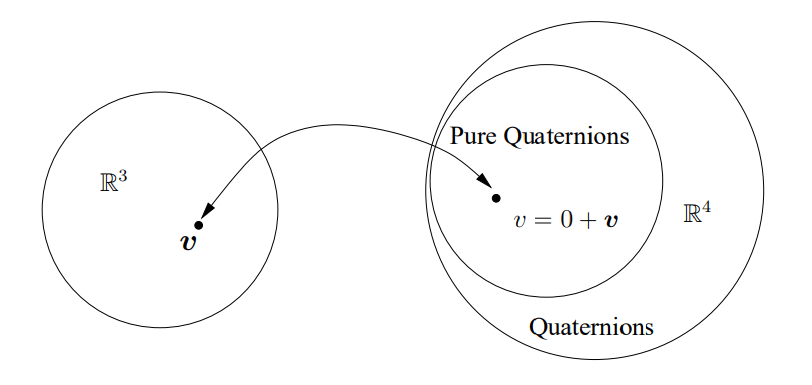
\includegraphics[width=1.0\textwidth]{figures/r3.png}
	\caption{$\mathbb{R}^3$ can be viewed as a subspace of quaternions called pure quaternions which have a real part of zero.}
	\label{f:r3}
\end{figure*}

Using the unit quaternion $q$ let us define a function $L_q:~\mathbb{R}^3 \rightarrow \mathbb{R}^3$ on vectors $\textbf{v} \in \mathbb{R}^3
$:
\begin{align}
L_q(\textbf{v}) &= q\textbf{v}q^* \nonumber \\
&= (q_0^2 - ||\textbf{q}||^2)\textbf{v} + 2(\textbf{q}\cdot\textbf{v})\textbf{q} + 2q_0(\textbf{q} \times \textbf{v}). 
\label{eq:Lq}
\end{align}

Two observations to note are that first, the operation \eqref{eq:Lq} does not modify the length of the vector $\textbf{v}$:
\begin{align*}
||L_q(\textbf{v})|| &= ||q\textbf{v}q^*||  \\
&= |q| \cdot ||\textbf{v}|| \cdot |q^*| \\
&= ||\textbf{v}||. 
\end{align*}
And second, the direction of $\textbf{v}$, if along $\textbf{q}$, is left unchanged by the function. To verify let $\textbf{v} = k\textbf{q}$
\begin{align*}
L_q(\textbf{v}) &= q(k\textbf{q})q^*  \\
&= (q_0^2 - ||\textbf{q}||^2)k\textbf{q} + 2(\textbf{q}\cdot k\textbf{q})\textbf{q} + 2q_0(\textbf{q} \times k\textbf{q}) \\
&= k(q_0^2 + ||\textbf{q}||^2)\textbf{q} \\
&= k\textbf{q}.
\end{align*}
Using our insights from complex numbers this lets us guess that the function \eqref{eq:Lq} acts like a rotation about $\textbf{q}$.

\begin{theorem}
For any unit quaternion
\begin{equation}
q = q_0 + \textbf{q} = \mbox{cos}\frac{\theta}{2} + \mathbf{\hat{u}}\mbox{sin}\frac{\theta}{2},
\label{eq:unitquat}
\end{equation}
and for any vector $\textbf{v} \in \mathbb{R}^3$ the result of the function
\begin{equation*}
L_q(\textbf{v}) = q\textbf{v}q^*
\end{equation*}
on $\textbf{v}$ is equivalent to a rotation of the vector through an angle $\theta$ about $\mathbf{\hat{u}}$ as the axis of rotation.
\end{theorem}

\begin{proof}
Given a vector $\textbf{v} \in \mathbb{R}^3$, we decompose it as $\textbf{v} = \textbf{a} + \textbf{n}$, where $\textbf{a}$ is the component along the vector $\textbf{q}$ and $\textbf{n}$ is the component normal to $\textbf{q}$. 
Then we show that under the function $L_q$, $\textbf{a}$ is invariant, while $\textbf{n}$ is rotated about $\textbf{q}$ through an angle $\theta$. 

Earlier we showed that $\textbf{a}$ is invariant under $L_q$ so let us see how $L_q$ transform $\textbf{n}$.
\begin{align*}
L_q(\textbf{n}) &= (q_0^2 - ||\textbf{q}||^2)\textbf{n} + 2(\textbf{q} \cdot \textbf{n})\textbf{q} + 2q_0(\textbf{q} \times \textbf{n}) \\
&= (q_0^2 - ||\textbf{q}||^2)\textbf{n} + 2q_0(\textbf{q} \times \textbf{n}) \\
&= (q_0^2 - ||\textbf{q}||^2)\textbf{n} + 2q_0||\textbf{q}||(\mathbf{\hat{u}} \times \textbf{n}),
\end{align*}
where in the last step we introduced $\mathbf{\hat{u}} = \textbf{q}/||\textbf{q}||$.
Let $\textbf{n}_{\bot} = \mathbf{\hat{u}} \times \textbf{n}$ to get
\begin{equation}
L_q(\textbf{n}) = (q_0^2 -||\textbf{q}||^2)\textbf{n} + 2q_0||\textbf{q}||\textbf{n}_{\bot}.
\label{eq:p11}
\end{equation}
Also note that $\textbf{n}_{\bot}$ and $\textbf{n}$ have the same length:
\begin{equation*}
||\textbf{n}_{\bot}|| = ||\textbf{n} \times \mathbf{\hat{u}}|| = ||\textbf{n}|| \cdot ||\mathbf{\hat{u}}||\mbox{sin}\frac{\pi}{2} = ||\textbf{n}||.
\end{equation*}
Then rewriting \eqref{eq:p11} we arrive at
\begin{align*}
L_q(\textbf{n}) &= \left( \mbox{cos}^2 \frac{\theta}{2} - \mbox{sin}^2 \frac{\theta}{2} \right) \textbf{n} + \left( 2\mbox{cos} \frac{\theta}{2} \mbox{sin} \frac{\theta}{2} \right) \textbf{n}_{\bot} \\
&= \mbox{cos}~\theta \textbf{n} + \mbox{sin}~\theta \textbf{n}_{\bot}.
\end{align*}
The resulting vector is a rotation of $\textbf{n}$ through an angle $\theta$ in the plane defined by $\textbf{n}$ and $\textbf{n}_{\bot}$.
\end{proof}
















\chapter{Introduction To Convolutional Neural Networks}
The Convolutional Neural Network (CNN) is a well-known deep learning architecture that was loosely inspired by the natural visual perception mechanism of some living organisms.
This comes from a paper by Hubel and Wiesel \cite{hubel1968receptive} in 1959 where they found that their were specific cells in the visual cortex of animals that were responsible for detecting light in the receptive field, which eventually won them a Nobel Prize. 
It was not until 1990 that LeCun et al. \cite{lecun1990handwritten} released the crucial paper that would establish modern framework for CNNs. 
Their model was a multiple layer neural network called LeNet-5 that could classify 28x28 greyscale hand written digit images with very high accuracy. 
As seen in Fig.~\ref{f:lenet} LeNet-5 has multiple layers and can be trained with the back-propagation algorithm \cite{hecht1988theory}, but used a low number of parameter values for its size. 
To achieve this LeNet-5 used two core components, which we will discuss in the next section.

\begin{figure}[h!]
	\centering
		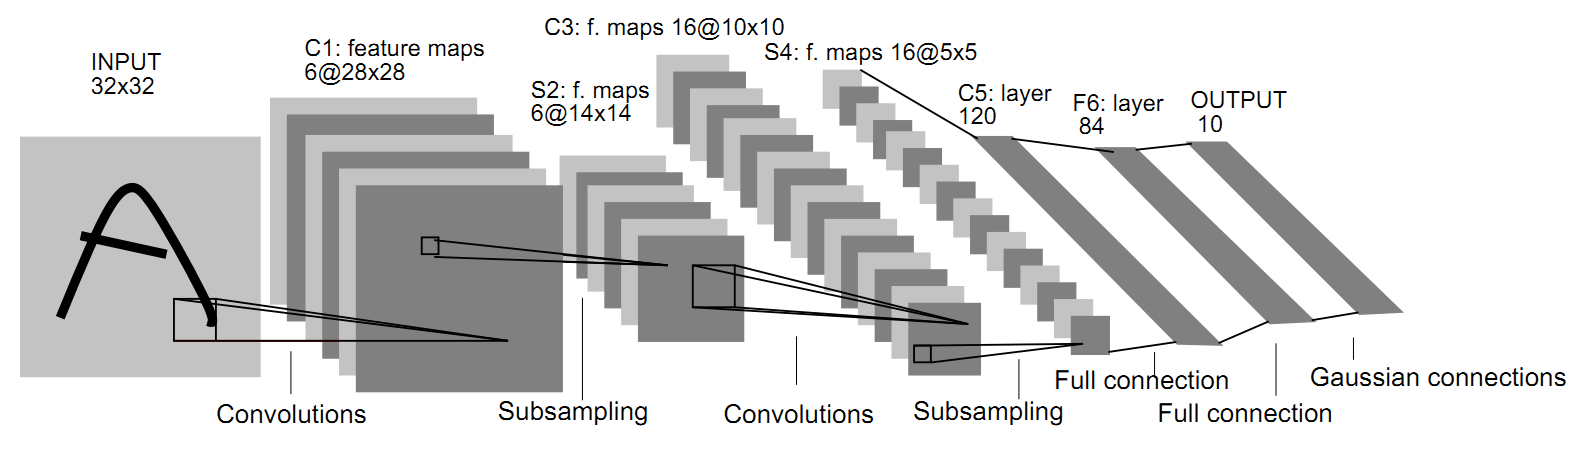
\includegraphics[width=0.95\textwidth]{figures/lenet5.png}
	\caption{The architecture for LeNet-5, which is composed of repeating convolution and pooling layers.}
	\label{f:lenet}
\end{figure}

\section{Basic CNN Components}
While there are many different layer types in current literature, here we will focus on the two introduced in LeNet-5, which are still used today along with some variants of them. 

\subsection{Convolutional Layer}
The first is the convolution layer. 
Its purpose is to learn feature representations of the inputs. 
Each convolution layer has a specified number of kernels where each kernel is unique as to generate a distinct feature map. 
Each neuron of a feature map is connected to a region of neighboring neurons in the previous layer. 
The size of the connection is known as the kernel size or the receptive field size. 
The feature map is obtained by first convolving the input with the kernel and then applying an element-wise nonlinear activation function on the result. 
Because it is a convolution operation each kernel is shared with all spatial locations of the input. 
This spatial weight sharing is what creates the low parameter number compared to a regular neural network which fully connects all inputs and outputs. 
It also allows the CNN to take advantage of the underlying structure in images. 
Topological information, i.e., spatial information about the structure in an image, such as adjacency and rotations are also taken into account. 
The equation for finding the feature value at location $(i,j)$ in the $k^{th}$ feature map of the $l^{th}$ layer, $z^l_{i,j,k}$ is
\begin{equation}
z^l_{i,j,k} = {\textbf{w}^l_k}^T \textbf{x}^l_{i,j} + b^l_k
\label{eq:convbasic}
\end{equation}
where $\textbf{w}^l_k$ and $b^l_k$ are the weight vector, or convolution kernel, and the bias term of the $l^{th}$ layer respectively, and $\textbf{x}^l_{i,j}$ is the input patch centered at location $(i,j)$ of the $l^{th}$ layer. 
An example of this operation can be seen in Fig.~\ref{f:convolution}. 
After the convolution is applied the result is then put through the nonlinear activation function:
\begin{equation}
a^l_{i,j,k} = a(z^l_{i,j,k})
\label{eq:activationbasic}
\end{equation}
where $a(\cdot)$ is the nonlinear activation function. 
We will discuss different activation functions in great detail in Chapter \ref{StateOfTheArt}.

\begin{figure}[h!]
	\centering
		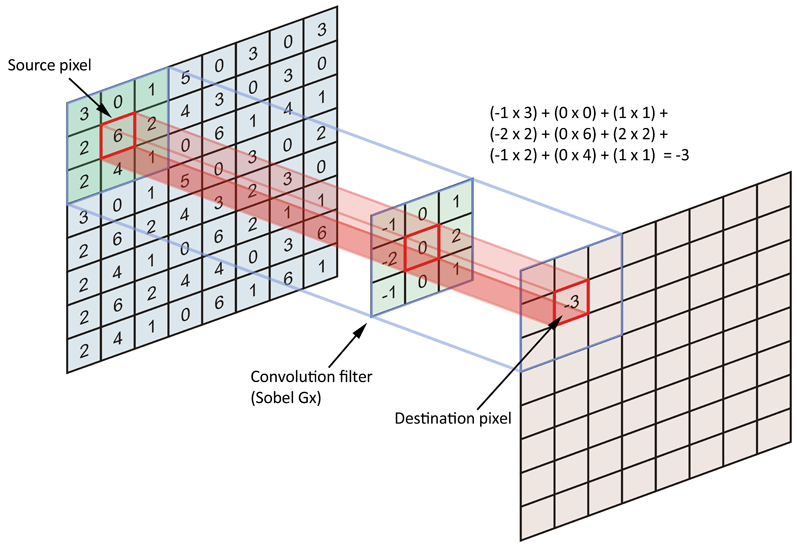
\includegraphics[width=0.95\textwidth]{figures/convolution.png}
	\caption{Convolution operation performed on a single feature location and one convolution kernel \cite{convolution}.}
	\label{f:convolution}
\end{figure}


\subsection{Pooling Layer}
The other key layer is the pooling layer shown in Fig.\ref{f:lenet} as subsampling. 
The pooling layer comes after a convolution layer and it performs a reduction in the resolution of the feature map. 
This layer works typically with two arguments: the spatial size of the pooling window $F$ and the stride, or shift per operation, $S$.
It is accomplished in a similar manner to convolution, starting at the top right a window of size $F \times F$ is grabbed.
From this window the pooling function is used, which is commonly a \textbf{MAX} function.
The window then moves over by $S$ pixels and the above operation happens again.
This is repeated until the whole image is covered.
For example, if one chooses $F = 2$ and $S = 2$ they will be selecting the maximum pixel in a $2 \times 2$ window and moving 2 pixels over exactly as shown in Fig.~\ref{f:maxpool}.
Note that this reduces the original image by a factor of $F = 2$.
This serves the purpose of reducing the number of multiplications the architecture must perform and also aims to achieve shift invariance. 
We will discuss different pooling techniques in Chapter \ref{StateOfTheArt}.

\begin{figure}[h!]
	\centering
		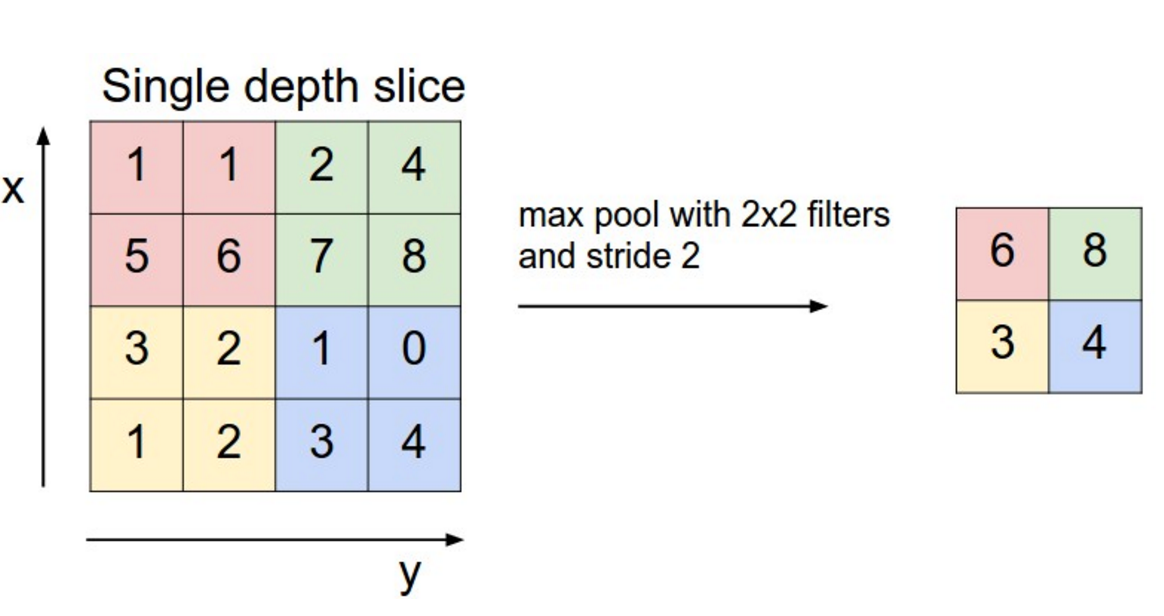
\includegraphics[width=0.95\textwidth]{figures/maxpool.png}
	\caption{Example max pooling operation with a size of 2x2. A 2x2 window is moved over the input with a stride of 2 and the maximum value of the window is taken \cite{maxpooling}.}
	\label{f:maxpool}
\end{figure}

There is also the inverse of pooling, often called upsampling, that will increase the resolution of the feature maps.
There are several cases where this is a desired effect which we will discuss later.


\subsection{CNN Common Tasks}
The last layers of LeNet-5 are fully connected layers like that of a regular Feed-Forward Neural Network (FNN), sometimes called Multilayer Perceptrons \cite{rumelhart1985learning}. 
The second to last layer is sometimes called a decision layer as it takes the outputs from the feature mapping and combines them together. 
The last layer is a fully connected layer of size 10, which corresponds to the number of classes in that particular data set. 
The classes, which are digits numbered 0 through 9, are represented as a `one hot' vector, meaning that if the class is the digit `0' the first element of the output vector should be 1 and the rest should be 0. 
This can be thought of as a probability distribution on the classes. 
This is an important representation because it allows one to use loss functions that minimizes the differences of distributions opening up many potential loss functions.
This was the common use case for CNNs for a while, given an image predict a distribution over a set of classes. 
This task is known as \textit{classification}. 

Recently CNNs have seen use in another area known as \textit{semantic segmentation}.
Semantic segmentation, also sometimes just called segmentation, is the process of partitioning an image into multiple segments, or sets of pixels. 
More precisely, segmentation is the process of assigning a class from our classification set to each pixel, or potentially area of pixels, in an image. 
Unlike classification, the output of this CNN would typically be in the form of an image.
Typically the network will output a distribution over a set of classes \textit{per pixel} and then the pixel is labeled with the class with the highest probability. 
There are many applications where image classification alone does not giving enough information and one needs pixel-level labels. 
Examples include: detecting road signs \cite{maldonado2007road}, detecting tumors in medical imaging \cite{li2015automatic, lyksborg2015ensemble, kainz2015semantic, havaei2017brain}, detecting objects of interest from satellite photos \cite{chen2013vehicle}, finding pedestrians \cite{du2016fused}, and many more. 
Having pixel level labels allows multiple objects of different classes to be detected in one image compared to image level labels where there is a single output per image.

In recent years, CNNs have obtained state of the art results on almost all classification and segmentation data sets. 
The improvements in CNNs have come from a few different areas including better computers, improvements to initialization of network weights, and specific architectures to combat problem areas of deep networks. 
In this next chapter we will go through a list of improvements and key papers.  
\chapter{State of the Art}\label{StateOfTheArt}
In this chapter we will go over the latest improvements for CNNs. 
They range from the activation function used within each neuron to major architecture overhauls from the original LeNet-5.


\section{Recent Advances in Training Neural Networks}\label{s:NNAdvances}

\subsection{Activation Functions}
There have been many recent papers on improving the results of NNs in general. One focus has been on the activation functions used inside the network. The current trend has been using activation functions that are non-saturated, meaning they do not have very small derivatives at large input values. All mentioned activation functions can be seen in Fig.~\ref{f:activations}.

\paragraph{ReLU:}
The most notable non-saturated activation function is the rectified linear unit (ReLU) \cite{nair2010rectified}. This is defined as:
\begin{equation}
f(x) = \mbox{max}(0,x).
\label{e:relu}
\end{equation}
The benefits of this unit include: faster calculation since the max($\cdot$) operation is faster than sigmoid or tanh, it creates sparsity in the hidden units by giving true zero values often to help sparse representations form, and does not suffer from vanishing gradients in deep models. ReLU has been shown to work better than sigmoid or tanh in several tasks and shows fast convergence even without pretraining \cite{glorot2011deep,krizhevsky2012imagenet,zeiler2013rectified,maas2013rectifier}.

\paragraph{LReLU:}
The ReLU has zero gradient whenever its inputs add to a negative value or when a large gradient changes the weights to large negatives value making future input into the unit always have a negative value. These units will never be updated and learning will not occur, which can be a problem. Mass \textit{et al}. \cite{maas2013rectifier} found a solution to this by introducing a non zero component to the ReLU when the input is negative. They called this unit the Leaky ReLU as it 'leaks' a positive gradient on the negative side of its graph by having a very small slope. This leaky ReLU or LReLU is defined as:
\begin{equation}
f(x) = \mbox{max}(0,x) + \lambda ~\mbox{min}(0,x)
\label{e:lrelu}
\end{equation}
where $\lambda \in (0,1)$ and is predefined per model. This unit allows for small gradients when the unit is not active, which helps the problems of the ReLU unit.

\paragraph{PReLU:}
Rather than trying to find an optimal value for $\lambda$ in the LReLU, He et al. \cite{he2015delving} introduced the Parametric ReLU which adapts the $\lambda$ during training. It is defined as:
\begin{equation}
f(x) = \mbox{max}(0,x) + \lambda_k ~\mbox{min}(0,x)
\label{e:prelu}
\end{equation}
where $\lambda_k$ is the $k$-th channel. Since the number of parameters in networks is often very large compared to the number of total channels, the extra computational cost to learn the values of $\lambda_k$'s is not much.

\paragraph{ELU:}
Next is the Exponential Linear Unit (ELU) \cite{clevert2015fast}. ELUs are similar to the above mentioned units, but they have a saturating function on their negative side. The saturation function decreases the variation of the units if they are not activated, which gives those units a chance to update while making them more robust to noise. The ELU function is defined as:
\begin{equation}
f(x) = \mbox{max}(0,x) + \mbox{min}(0,\lambda(e^{x}-1))
\label{e:elu}
\end{equation}
where $\lambda$ is predefined as in the LReLU.

\paragraph{PELU:}
A natural extension of the ELU is the Parametric ELU \cite{trottier2016parametric}. Unlike the PReLU which learns one parameter to modify the LReLU, the PELU learns two parameters during training to modify the ELU. This gives the network more control over the vanishing gradients. The PELU is defined as:
\begin{equation}
f(x) = \mbox{max}(0,\frac{a}{b}x) + \mbox{min}(0,a(e^{x/b}-1))
\label{e:pelu}
\end{equation}
where $a,b > 0$. Both $a$ and $b$ change the slope of the linear function together, $b$ effects the scale of the exponential decay, and $a$ is the saturation point in the negative side of the function. In \cite{trottier2016parametric} it is shown that PELU does a better job than all the above functions in several different models and data sets.

\begin{figure}[h!]
	\centering
		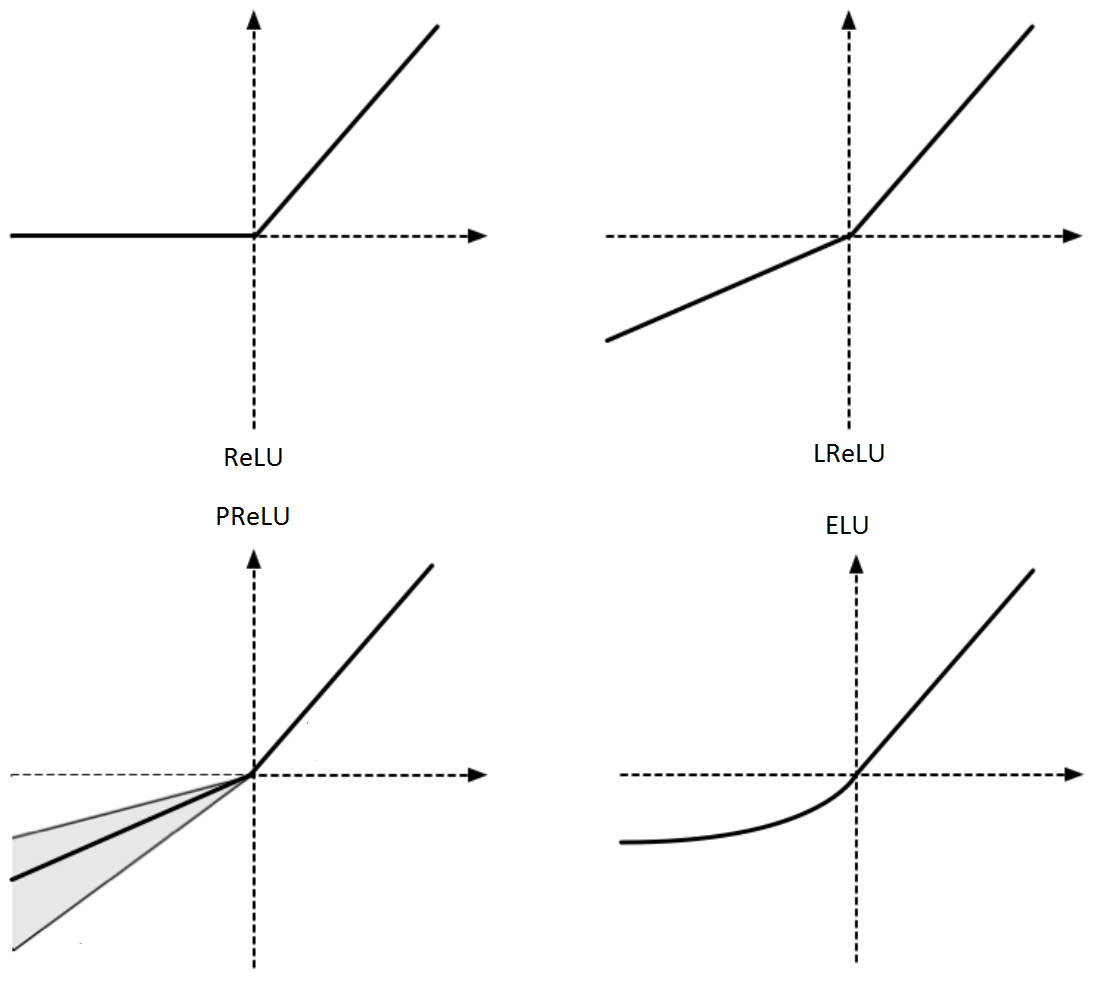
\includegraphics[width=0.85\textwidth]{figures/activations.png}
	\caption{Examples of some of the discussed activation functions. From top to bottom and left to right: ReLU, LReLU, PReLU, and ELU. \cite{}}
	\label{f:activations}
\end{figure}


\subsection{Regularization}
Some of the biggest improvements to NNs have been through regularizing the network in different ways to prevent overfitting.

\paragraph{Dropout:}
Introduced by Hinton \textit{et al.} \cite{hinton2012improving}, Dropout has shown to be very effective at improving network results and reducing overfitting. In their paper Dropout is applied to fully-connected layers where the output of the Dropout layer is 
\begin{equation}
\textbf{y} = \textbf{r} \ast a(\textbf{W}^T\textbf{x}), 
\label{eq:dropout}
\end{equation}
where $\textbf{x} = [x_1,x_2,...,x_n]^T$ is the input to the fully-connected layer, $a(\cdot)$ is an activation function, $\textbf{W}$ is the weight matrix, $\ast$ is an element-wise multiplication, and $\textbf{r}$ is a binary vector whose elements are independently drawn from a Bernoulli distribution with parameter $p$. This means that at every update to the network, each neuron has a $p$ chance of getting multiplied by zero. Dropout usually prevents the network from becoming too reliant on a few neurons and helps the network generalize by spreading feature information. Some extensions to Dropout have been proposed like in \cite{wang2013fast} where a method to improve the speed of training while using Dropout are introduced. Similar to the learned parameters of the activation functions, \cite{ba2013adaptive} learn the $p$ in the Dropout distribution adaptively. Finally, in \cite{tompson2015efficient} they modify Dropout with CNNs specifically in mind by extending the Dropout value across the entire feature map, meaning that during training each feature map has a $p$ chance of being completely ignored for each update step. They call this method Spatial Dropout and it seems to help the network learn more general features, which improves results on limited size data sets.

\paragraph{Batch Normalization:}
It is standard practice to normalize data to have zero-mean and unit variance before feeding it into a NN, but as the data goes through the network, especially deep networks, the data will lose this property. This change to the input distribution is known as internal covariance shift. To keep data normed through the network \cite{ioffe2015batch} introduced an efficient method called Batch Normalization (BN). BN works by normalizing the mean and variance of each layers input using each batch rather than the entire training set. To demonstrate BN, let $\textbf{x} = [x_1,x_2,...,x_n]^T$ be a $n$ dimensional input to a layer. The $k$-th dimensions is normalized by:
\begin{equation}
\hat{x}_k = (x_k - \mu_{B})/\sqrt{\sigma^2_B + \epsilon}
\label{eq:BN1}
\end{equation}
where $\mu_{B}$ and $\sigma^2_B$ are the mean and variance of the batch respectively and $\epsilon$ is some small constant value that will guarantee the root term is always defined. Finally the input $\hat{x}_k$ is further transformed:
\begin{equation}
y_k = \mbox{BN}_{\alpha,\beta}(x_k) = \alpha \hat{x}_k + \beta
\label{eq:BN2}
\end{equation}
where $\alpha$ and $\beta$ are parameters learned during training. There are many benefits to using BN. By reducing internal covariance shift the network will converge faster. By making sure no inputs get too large or small BN makes it possible to use saturating activation functions without fear of getting stuck in a saturating section and having vanishing gradients. This is very important when training GANs, which are extremely sensitive to the issues BN addresses.

\subsection{Architecture Improvements}
There are a couple of recent architecture improvements to NNs in general that inspired some of the newer ideas in segmentation. The first was introduced in \cite{lin2013network} where they use fully connected layers on the outputs of each convolution operation called Network-in-network. The idea was an alternative to stacking multiple convolutional layers (each with a number of their own filters) to get deepness in a neural network model, by replacing each filter with a multi-layer perceptron, which is essentially a small neural network that slides across the image like a convolutional filter. The math works out so that a $1\times 1\times U$ convolution filter convolved across a $V$-channel image emulates a $U\times V$ matrix multiplied by each $V$-channel pixel, which is the same as running a single-layer neural network across every pixel of your input as if each pixel were an example vector in a training set. Chaining together such $1\times 1\times U$ convolutions, you get the same result as if running a many-layered neural network at each input pixel of $V$ channels.  The idea from the paper was to turn a convolution filter which is a generalized linear model, into a non-linear model. It allows the network to combine channels from previous layer in a non-linear fashion, which can lead to more advanced features.

Google's team was inspired by the Network-in-network paper and saw the power of using the 1x1 convolutions not only for non-linearaity, but to reduce computational burden of deep models by using the cross-channel pooling aspect to reduce their feature maps before convolution layers. In \cite{szegedy2015going} Christian Szegedy and his team introduced the Inception module as seen in Fig.\ref{f:inceptionblock}. 

\begin{figure}[h!]
	\centering
		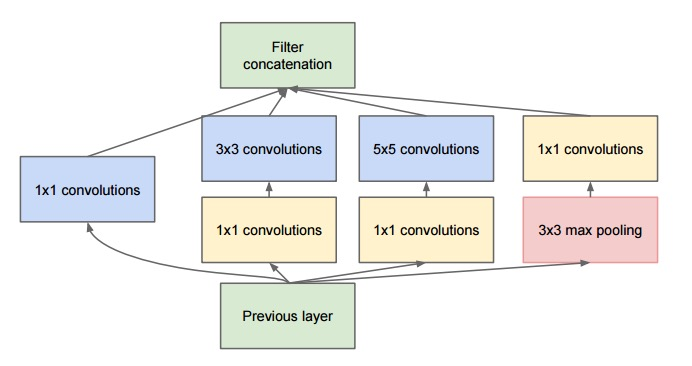
\includegraphics[width=1.0\textwidth]{figures/inceptionblock.png}
	\caption{An inception block from \cite{szegedy2015going}. Notice the 1x1 convolutions before the 3x3 and 5x5 convolutions are reducing the number of feature channels. This reduces the number of multiplications that must be performed.}
	\label{f:inceptionblock}
\end{figure}

Another work that focused on fixing the vanishing gradient problem of deep networks was Residual Nets (ResNets) \cite{he2015deep} where they used what is now called shortcut connections. These connections were inspired by Long Short Term Memory (LSTM) units, a type of recurrent neural network unit that feeds information back into itself with weighted gates. Instead of using weighted gates shortcut connections pass information with the identify function so it is untransformed. This means that the activation of deep units can be written as the sum of the activation of some shallower unit and a residual function, which is a series of network layers. Or to put simply, the input to a layer group is added to the output of that layer group. This is called a Residual Block and can be seen in Fig.\ref{f:resblock}. By stacking these residual blocks together one gets a fully residual model. This design allows the gradients to be directly propagated to shallower units allowing for networks of 100s of layers to be trained. 
\begin{figure}[h!]
	\centering
		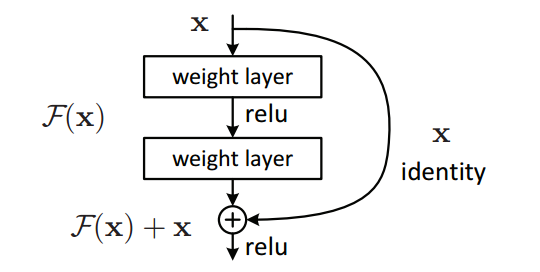
\includegraphics[width=0.80\textwidth]{figures/resblock.png}
	\caption{A residual block from \cite{he2015deep}.}
	\label{f:resblock}
\end{figure}


\section{Recent Advances in CNNs for Semantic Segmentation}\label{s:RecentAdvsCNNs}
The area of segmentation has recently seen many improvements using methods mentioned in the Section \ref{s:NNAdvances}. The highlight papers that brought big improvements to the area and that inspired the work in this thesis will be discussed each in their own section.

\subsection{Fully Convolutional Networks for Semantic Segmentation}
In \cite{long2015fully} Long \textit{et al}. used 1x1 convolutional kernels at the end of their network, instead of a fully connected layer, to produce a dense heatmap prediction of their classes as seen in Fig.~\ref{f:fcn1}. They then used \textit{backwards convolution}, sometimes called \textit{deconvolution} or \textit{transposed convolution}, with some input stride to upsample this dense heatmap back up to the original input image size. By using this method to upsample they achieve a non-linear learned upsampling. Backwards convolution works by taking the input image and padding zeros between the pixels based on the stride of the convolution shown in Fig.~\ref{f:deconv}. The result is a segmentation of classes of the same size as the input image trained fully end to end. 
\begin{figure}[h!]
	\centering
		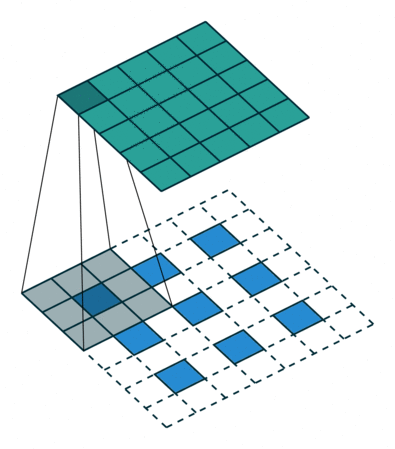
\includegraphics[width=0.50\textwidth]{figures/padding_strides_transposed.png}
	\caption{Backwards convolution with a stride of 2 upsampling a 3x3 image to a 5x5 image. Notice the 3x3 image is padded with zeros, the white tiles. The shaded grey area is the actual convolution kernel, which is learned during training.}
	\label{f:deconv}
\end{figure}
\begin{figure}[h!]
	\centering
		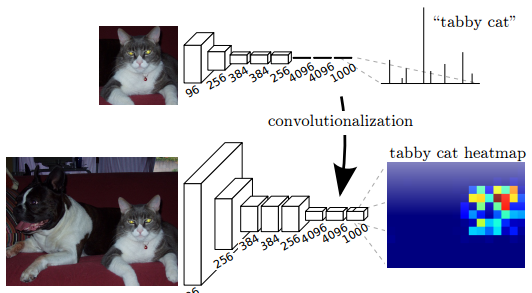
\includegraphics[width=0.90\textwidth]{figures/fcn1.png}
	\caption{Transforming fully connected layers into convolution layers enables a classification net to output a heatmap \cite{long2015fully}. This is achieved by using 1x1 convolutions instead of fully connected layers and will produce a tiny heatmap of classes. This change also make the network become independent of input image size.}
	\label{f:fcn1}
\end{figure}
However, the results are very coarse even with learned upsampling from the deconvolution layers. To remedy this they used the idea of short connections to forward information from shallow layers, upsample them to the correct matching size of the current layer, and then combine them with the current layer. This adds the finer grain detail that the shallow layers possess that get lost after pooling operations. Some of the different architectures can be seen in Fig.~\ref{f:fcn2}. Their three models used increasing number of short connections, which increased the accuracy with each additional connection. It is important to note that in this paper they used weights from a pre-trained classification network and only the new backward convolution layers and onward were learned from the segmentation maps. 
\begin{figure}[h!]
	\centering
		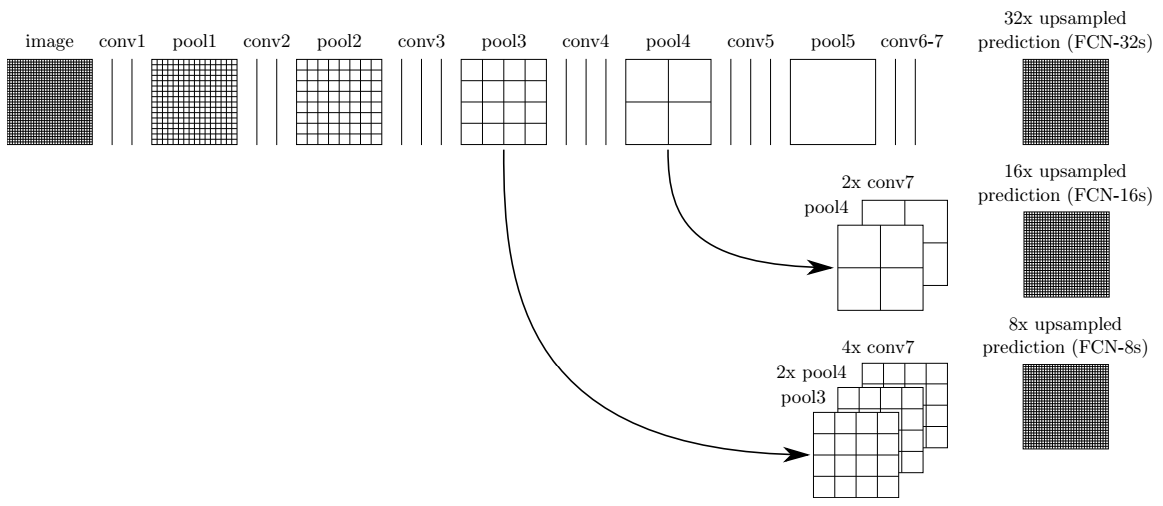
\includegraphics[width=1.0\textwidth]{figures/fcn2.png}
	\caption{Three different architectures from \cite{long2015fully}. The first uses no short connections, the second forwards information from pool4, and the third forwards information from both pool3 and pool4.}
	\label{f:fcn2}
\end{figure}

\subsection{U-Net: Convolutional Networks for Biomedical Image Segmentation}\label{s:unet}
Ronneberger \textit{et al.} in \cite{ronneberger2015u} directly mention that they are trying to improve upon results from \cite{long2015fully}. Since their application is medical segmentation the maps cannot be coarse so their aim is to improve in that area specifically as well as allowing for the network to be trained end-to-end, or no loading pre-trained weights. Their architecture consists of a contracting path (left side) into an expansive path (right side). The left side is a typical CNN and the right side is the inverse of the left, using deconvolution to upsample. Heavy use of short connections is used by forwarding information from every layer from the first half of their model to the matching size layer of the second half where it is then concatenated as shown in Fig.~\ref{f:unet}. This short connection from every layer in the contracting side differs from Long \textit{et al}., which used only two at most.
\begin{figure}[h!]
	\centering
		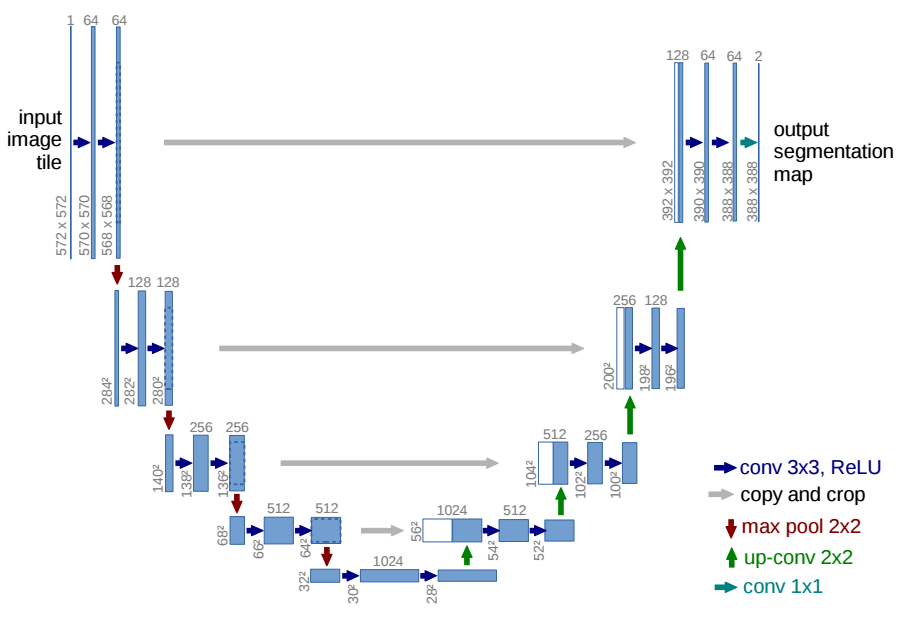
\includegraphics[width=1.0\textwidth]{figures/unet.png}
	\caption{U-Net architecture (example for 32x32 pixels in the lowest resolution). Each blue box corresponds to a multi-channel feature map. The number of channels is denoted on top of the box. The x-y-size is provided at the lower left edge of the box. White boxes represent copied feature maps. The arrows denote the different operations. \cite{ronneberger2015u}.}
	\label{f:unet}
\end{figure}
They also use an overlapping tile prediction strategy, which combats the edge artifacts from padding convolution operations with zeros. This means the prediction is only done on some middle portion of the input image.  

\subsection{Learning Iterative Processes with Recurrent Neural Networks to Correct Satellite Image Classification Maps}\label{PDERNN}
Maggiori \textit{et al.} at Inria in  \cite{maggiori2016learning} introduced a post processing network RNN whose sole purpose was to enhance segmentation results from a CNN. They formulate a generic partial differential equation (PDE) diffusion process applied to a map $u$, which is the segmentation result from the first network. They take as input a score map $u_k$ (for class $k$) and an arbitrary number of feature maps ${g_1,g_2,...,g_p}$ derived from image $I$. Then convolution kernels ${M_1,M_2,...}$ and ${N_1,N_2,...}$ are applied to the heat map $u_k$ and the features $g_j$ derived from image $I$ respectively. These filters are learned during training. These feature maps from applying these convolutions are gathered into a set:
\begin{equation}
\Phi(u_k,I) = \left\{ M_i \ast u_k, ~N_l^j \ast g_j(I);~\forall i,j,l\right\}.
\label{eq:cnnrnnset}
\end{equation}
Then $u_k$ can be expressed as changing in time as
\begin{equation}
\frac{\partial u_k(x)}{\partial t} = f_k(\Phi(u_k,I)(x)),
\label{eq:cnnrnn1}
\end{equation}
where $f_k$ is a function that takes as input the values of all the features in $\Phi(u_k,I)$ at an image point $x$ and combines them. Since it is discretized in time it takes the form:
\begin{equation}
u_{k,t+1}(x) = u_{k,t}(x) + \delta u_{k,t}(x),
\label{eq:}
\end{equation}
where $\delta u_{k,t}$ is the overall update of $u_{k,t}$ at time $t$. This $\delta u_{k,t}$ is the value that the post processing network will be trying to approximate using convolution results fed into a fully connected layer, known to be able to approximate any function, shown in Fig.\ref{f:cnnrnn1}. They do this in an iterative fashion where the update $u_{k,t+1}(x)$ is fed into the same network with shared weights $N$ number of times. They use $N = 5$ in their paper. This iterative step is a recurrent network and has a couple of advantages. First the weight sharing cuts the number of parameters down by a factor of $N$, making it easier to train. And second, the weight sharing is more physically realistic to a PDE. At each update the physics should remain unchanged, which would not be modeled properly if each iteration had a unique set of weights. An example of the complete RNN can be seen in Fig.\ref{f:cnnrnn2}.
\begin{figure}[h!]
	\centering
		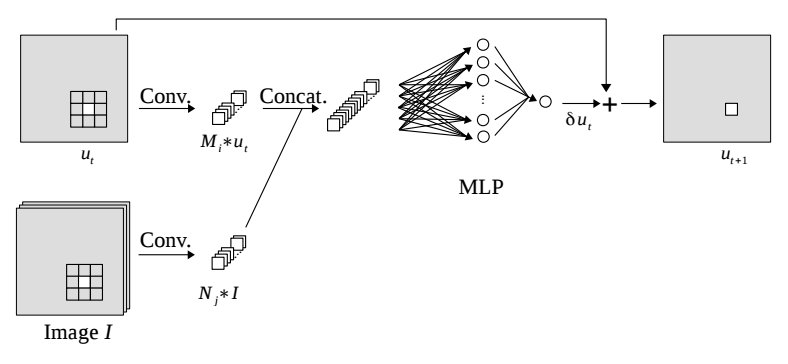
\includegraphics[width=1.0\textwidth]{figures/cnnrnn1.png}
	\caption{One iteration of the RNN represented as common neural network layers. The block approximates $\delta u_{k,t}$ and then adds it to $u_{k,t}$ to estimate $\delta u_{k,t}$. \cite{maggiori2016learning}}
	\label{f:cnnrnn1}
\end{figure}
\begin{figure}[h!]
	\centering
		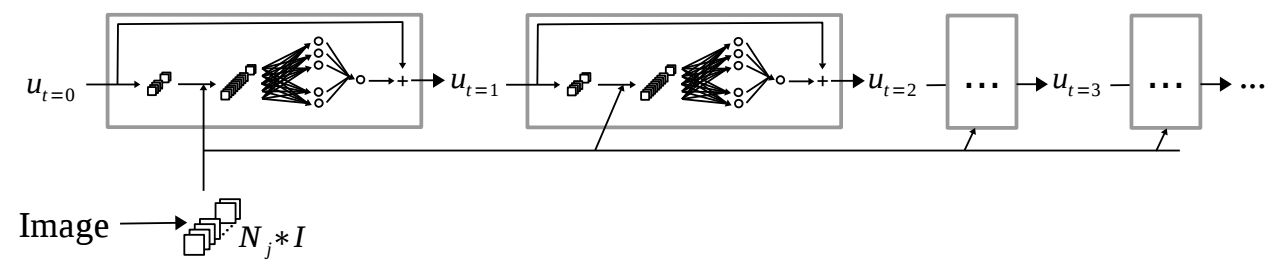
\includegraphics[width=1.0\textwidth]{figures/cnnrnn2.png}
	\caption{The whole RNN shown by multiple blocks from Fig.\ref{f:cnnrnn1} with shared weights. \cite{maggiori2016learning}.}
	\label{f:cnnrnn2}
\end{figure}


\subsection{Semantic Segmentation using Adversarial Networks}
\subsubsection{Brief overview of GANs}
We will start with a brief overview of the basics of a Generative Adversarial Network (GAN). Goodfellow \textit{et al.} introduced GANs in \cite{goodfellow2014generative} as a new way to estimate generative models, which are models that generate new data with parameters significantly smaller than the amount of data we train them on. So the models are forced to discover and efficiently internalize the essence of the data in order to generate it. 

The basic idea of GANs is to set up a game or battle between two networks. One is the generator, which creates samples that are suppose to come from the training set distribution. The other network is the discriminator, which examines an input and predicts whether it is real or fake. For example let us say our generator takes a random array of numbers sampled from a Gaussian distribution and from that array produces an image. The discriminator takes in the image and does a binary classification of either real or fake, that is, to indicate whether it is from the generator distribution or not. To fool the discriminator, the generator must learn to create images that are indistinguishable from an image from the training set.

Let us write our two networks as two functions, each of which is differentiable with respect to its own inputs and respect to its own parameters. The discriminator is a function $D$ that takes $x$ as input and uses $\theta^D$ as parameters. The generator is a function $G$ that takes $z$ as input and uses $\theta^G$ as parameters. Each network has its own cost function that it seeks to minimize. The discriminator wants to minimize $J^D(\theta^D,\theta^G)$, but must do so while only controlling $\theta^D$. Likewise, the generator wants to minimize $J^G(\theta^D,\theta^G)$, but must do so while only controlling $\theta^G$. The solution to this coupled loss system is a Nash equilibrium \cite{ratliff2013characterization}. In this context a Nash equilibrium is a tuple $(\theta^D,\theta^G)$ that is a local minimum of $J^D$ with respect to $\theta^D$ and a local minimum of $J^G$ with respect to $\theta^G$.

GANs are notoriously hard to train and much work has been done on stabilizing training. The training process involves simultaneous minimization updates to each network. On each update two batches are sampled: a batch of $x$ values from the training set and a batch of $z$ values drawn from the generator. Then two gradient steps are made simultaneously: one updating $\theta^D$ to reduce $J^D$ and the other updating $\theta^G$ to reduce $J^G$. 

After the first GAN paper many people began working on the issue of training stability and trying to produce larger, more realistic images. The first major work released was Radford \textit{et al.} \cite{radford2015unsupervised} that showed some significant improvements. They saw that using Batch Normalization in both the discriminator and generator is a must, having any fully connected layers is a bad idea, and instead of pooling use a strided convolution.

The next big improvement came from Salimans \textit{et al.} \cite{salimans2016improved} where they did slight modifications to the learning procedure. Instead of having the generator trying to fool the discriminator, they proposed a new objective function. This objective requires the generator to generate data that matches the statistics of the real data. Then the discriminator is only used to specify which statistics are worth matching. They also showed that smoothing the training labels by making the discriminator target output from [0=fake image, 1=real image] to [0=fake image, 0.9=real image] improved training stability. Their modifications focused on the loss function of the GAN, which we will see in the next two papers is a large area for improvement.

Recently some new papers have come out showing using different loss functions can greatly improve training stability and results. The first is Arjovsky \textit{et al.} \cite{arjovsky2017wasserstein} where they use the Wasserstein distance instead of the typical Kullback-Leibler divergence. Unlike Kullback-Leibler divergence, which is not defined if they generator's learned distribution and the true distribution do not overlap well, the Wasserstein distance has a well defined gradient everywhere. The second is Mao \textit{et al.} \cite{mao2017lsgan} where they reformulate the discriminator's loss as a least squares loss. The binary loss typically used does not provide more weight from a sample right next to the decision boundary to a sample very far away from the boundary. Meaning that samples that barely pass the boundary are treated the same as samples that did very well. By using the least square loss they fix this issue.

\subsubsection{GANs for segmentation}
One major issue of using CNNs for segmentation is that spatial contiguity is typically lacking, meaning that the CNN does not use long range information when classifying a pixel. We have shown some ways to combat the issue above like forwarding information from earlier layers to later layers and in Section~\ref{PDERNN} where a RNN model is run on the CNNs results to improve boundary sharpness. Luc \textit{et al.} \cite{luc2016semantic} tackled this issue by formulating the segmentation task in a way that a GAN model could be trained to accomplish as shown in Fig.~\ref{f:seggan}. Their model consists of the segmentor, which is the generator in the typical GAN framework, and the adversarial network is the discriminator. The segmentor takes an image and produces a segmentation of class predictions. The discriminator is then fed the same image and either the actual ground truth segmentation label or the segmentor's segmentation. It then predicts if the segmentation is the ground truth label or the segmentor's result. By using a GAN they combine the conventional cross-entropy loss over each pixel with an adversarial term. The adversarial term encourages the segmentation model, which is the generator, to produce label maps that cannot be distinguished from the ground-truth labels of the training set by the discriminator. Since the adversarial model can assess the joint configuration of many label variables, it can enforce forms of higher-order consistency that cannot be enforced using pair-wise terms, nor measured by a per-pixel cross-entropy loss.

\begin{figure}[h!]
	\centering
		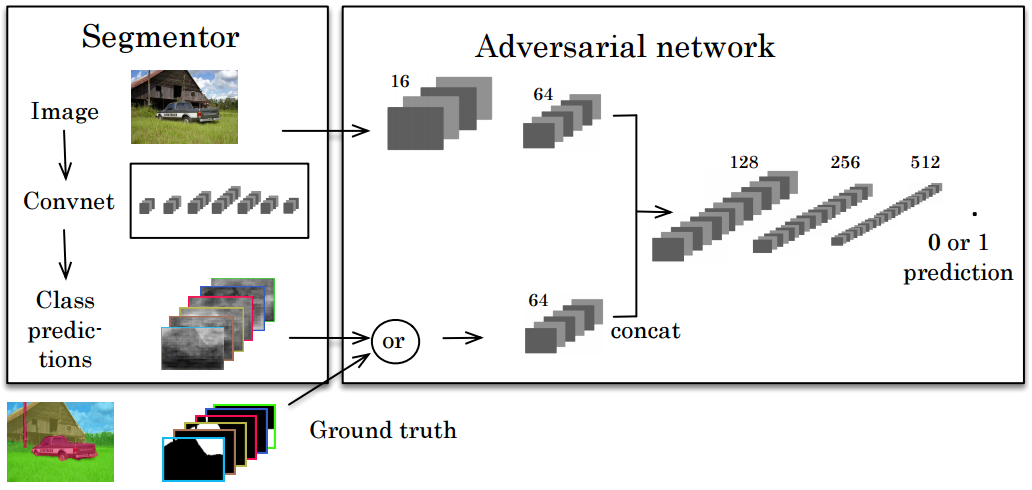
\includegraphics[width=1.0\textwidth]{figures/seggan.png}
	\caption{GAN formulation of semantic segmentation from \cite{luc2016semantic}. Left: segmentation net takes RGB image as input, and produces per-pixel class predictions. Right: Adversarial net takes label map as input and produces class label (1=ground truth, or 0=synthetic).}
	\label{f:seggan}
\end{figure}


\section{Open Questions}
There have been so many individual contributions to segmentation in the past couple of years, but combining these improvements into mixing architectures has not been studied. We intend to explore different combinations of good architectures to see if state-of-the-art can be improved. By creating the best mixed architecture we will not only have a better stand alone segmentation model, but we can hopefully further improve those results by both using it as a generator of a GAN model with untested loss functions for GAN segmentation and applying the iterative RNN process to the resulting segmentation heatmaps.

\chapter{Quaternion Networks}
At this point we have introduced the CNNs and their more recent advances as well as the basic concepts of quaternions.
In this chapter we will go through the motivation for constructing a neural network with quaternion values.
With the motivation in place we will then go through the known quaternion convolution operation before moving to our novel contributions of quaternion weight initialization and quaternion batch-normalization.
These pieces are then used to run some benchmark experiments and compared against real and complex valued networks.
The quaternion network outperforms both on two classification tasks and a segmentation task.


\section{Motivation and Related Work}
The ability of quaternions to effectively represent spatial transformations and analyze multi-dimensional signals makes them promising for applications in artificial intelligence.

One common use of quaternions is for representing rotation into a more compact form. 
PoseNet \cite{kendall2015posenet} used a quaternion as the target output in their model where the goal was to recover the $6-$DOF camera pose from a single RGB image.
The ability to encode rotations may make a quaternion network more robust to rotational variance.

Quaternion representation has also been used in signal processing.  
The amount of information in the phase of an image has been shown to be sufficient to recover the majority of information encoded in its magnitude by Oppenheim and Lin \cite{oppenheim1981importance}.
The phase also encodes information such as shapes, edges, and orientations.
Quaternions can be represented as a 2~x~2 matrix of complex numbers, which gives them a group of phases potentially holding more information compared to a single phase.

Bulow and Sommer \cite{bulow2001hypercomplex} used the higher complexity representation of quaternions by extending Gabor's complex signal to a quaternion one which was then used for texture segmentation.
Another use of quaternion filters is shown in \cite{sangwine2000colour} where they introduce a new class of filter based on convolution with hyper-complex masks, and present three color edge detecting filters. 
These filters rely on a three-space rotation about the grey line of RGB space and when applied to a color image produce an almost greyscale image with color edges where the original image had a sharp change of color.
More quaternion filter use is shown in \cite{shi2007quaternion} where they show that it is effective in the context of segmenting color images into regions of similar color texture. 
They state the advantage of using quaternion arithmetic is that a color can be represented and analyzed as a single entity (by assigning each color channel to an imaginary axis).
This comes from the structure of quaternion multiplication that was mentioned in Section \ref{s:quatConc}, which we will show holds for quaternion convolution in a convolutional neural network architecture as well in Section \ref{s:qc}.

A quaternionic extension of a feed forward neural network, for processing multi-dimensional signals, is shown in \cite{minemoto2017feed}.
They expect that quaternion neurons operate on multi-dimensional signals as single entities, rather than real-valued neurons that deal with each element of signals independently.
A convolutional neural network (CNN) should be able to learn a powerful set of quaternion filters for more impressive tasks.

Another large motivation is discussed in \cite{trabelsi2017deep}, which is that complex numbers are more efficient and provide more robust memory mechanisms compared to the reals \cite{bulow1999hypercomplex, sangwine2000colour, bulow2001hypercomplex}.
They continue that residual networks have a similar architecture to associative memories since the residual shortcut paths compute their residual and then sum it into the memory provided by the identity connection.
Again, given that quaternions can be represented as a complex group, they may provide an even more efficient and robust memory mechanisms.


\section{Quaternion Network Components}
This section will include the work done to obtain a working deep quaternion network. 
Some of the longer derivations are given in the Appendix.

\subsection{Quaternion Representation}
Recall the quaternion algebra presented in \ref{s:quatalg}.
Since we will be performing quaternion arithmetic using reals it is useful to embed $\mathbb{H}$ into a real-valued representation.
There exists an injective homomorphism from $\mathbb{H}$ to the matrix ring $M(4,\mathbb{R})$ where $M(4,\mathbb{R})$ is a 4x4 real matrix.
The 4~x~4 matrix can be written as
\begin{align}
\begin{bmatrix}
 a & -b & -c & -d \\ 
 b & a & -d & c \\
 c & d & a & -b \\
 d & -c & b & a 
\end{bmatrix}= &~~a
\begin{bmatrix}
 1 & 0 & 0 & 0 \\ 
 0 & 1 & 0 & 0 \\
 0 & 0 & 1 & 0 \\
 0 & 0 & 0 & 1 
\end{bmatrix}
\nonumber + b 
\begin{bmatrix}
 0 & -1 & 0 & 0 \\ 
 1 & 0 & 0 & 0 \\
 0 & 0 & 0 & -1 \\
 0 & 0 & 1 & 0 
\end{bmatrix}
\nonumber \\ &+ c
\begin{bmatrix}
 0 & 0 & -1 & 0 \\ 
 0 & 0 & 0 & 1 \\
 1 & 0 & 0 & 0 \\
 0 & -1 & 0 & 0 
\end{bmatrix}
\nonumber + d
\begin{bmatrix}
 0 & 0 & 0 & -1 \\ 
 0 & 0 & -1 & 0 \\
 0 & 1 & 0 & 0 \\
 1 & 0 & 0 & 0 
\end{bmatrix}.
\label{eq:m4r}
\end{align}
This representation of quaternions is not unique, but we will stick to the above in this paper.
It is also possible to represent $\mathbb{H}$ as $M(2,\mathbb{C})$ where $M(2,\mathbb{C})$ is a 2~x~2 complex matrix.

With our real-valued representation a quaternion real-valued $2D$ convolution layer can be expressed as follows. 
Say that the layer has $N$ feature maps such that $N$ is divisible by 4.
We let the first $N/4$ feature maps represent the real components, the second $N/4$ represent the $i$ imaginary components, the third $N/4$ represent the $j$ imaginary components, and the last $N/4$ represent the $k$ imaginary components.


\subsection{Quaternion Differentiability}
In order for the network to perform backpropagation the cost function and activation functions used must be differentiable with respect to the real, $i$, $j$, and $k$ components of each quaternion parameter of the network.
As the complex chain rule is shown in \cite{trabelsi2017deep}, we provide the quaternion chain rule which is given in the Appendix section \ref{a:diff}.


\subsection{Quaternion Convolution}\label{s:qc}
Convolution in the quaternion domain is done by convolving a quaternion filter matrix $\textbf{W}=\textbf{A}+\textit{i}~\textbf{B}+\textit{j}~\textbf{C}+\textit{k}~\textbf{D}$ by a quaternion vector $\textbf{h}=\textbf{w}+\textit{i}~\textbf{x}+\textit{j}~\textbf{y}+\textit{k}~\textbf{z}$. 
Performing the convolution by using the distributive property and grouping terms one gets
\begin{align}
\textbf{W}\ast \textbf{h} = &~(\textbf{A}\ast\textbf{w}-\textbf{B}\ast\textbf{x}-\textbf{C}\ast\textbf{y}-\textbf{D}\ast\textbf{z}) + \nonumber \\ 
&\textit{i}(\textbf{A}\ast\textbf{x}+\textbf{B}\ast\textbf{w}+\textbf{C}\ast\textbf{z}-\textbf{D}\ast\textbf{y}) + \nonumber \\
&\textit{j}(\textbf{A}\ast\textbf{y}-\textbf{B}\ast\textbf{z}+\textbf{C}\ast\textbf{w}+\textbf{D}\ast\textbf{x}) + \nonumber \\
&\textit{k}(\textbf{A}\ast\textbf{z}+\textbf{B}\ast\textbf{y}-\textbf{C}\ast\textbf{x}+\textbf{D}\ast\textbf{w}).
\end{align}
Using a matrix to represent the components of the convolution we have:
\begin{equation}
\begin{bmatrix}
 \mathscr{R}(\textbf{W}\ast \textbf{h}) \\ 
 \mathscr{I}(\textbf{W}\ast \textbf{h}) \\
 \mathscr{J}(\textbf{W}\ast \textbf{h}) \\
 \mathscr{K}(\textbf{W}\ast \textbf{h}) 
\end{bmatrix}
=
\begin{bmatrix}
 \textbf{A} & -\textbf{B} & -\textbf{C} & -\textbf{D}\\
 \textbf{B} & \textbf{A} & -\textbf{D} & \textbf{C} \\
 \textbf{C} & \textbf{D} & \textbf{A} & -\textbf{B} \\
 \textbf{D} & -\textbf{C} & \textbf{B} & \textbf{A} \\
\end{bmatrix}
\ast
\begin{bmatrix}
 \textbf{w} \\ 
 \textbf{x} \\
 \textbf{y} \\
 \textbf{z}
\end{bmatrix}
\label{eq:qconvolve2}
\end{equation}

An example is shown in Fig.~\ref{f:quatconv}, which is useful to visualize one of the main motivational factors of quaternions for CNNs.
Notice that the result of the quaternion convolution produces a unique linear combination of each axis per the result of a single axis.
This comes from the structure of quaternion multiplication and is forcing each axis of the kernel to interact with each axis of the image.
Real-valued convolution simply multiplies each channel of the kernel with the corresponding channel of the image.
The quaternion convolution is similar to a mixture of standard convolution and depthwise separable convolution from \cite{chollet2016xception}. 
This reuse of filters on every axis and combination may help extract texture information across channels as seen in \cite{shi2007quaternion}.
One can think in terms of a RGB where the greyscale can be the real axis and the RGB channels can be the $i, j, k$ axes.
Then a quaternion kernel convolved against this quaternion image will view the colors as a single entity, unlike standard real-valued convolution.
Since a quaternion can be thought of as a vector, the quaternion kernels and feature maps can be thought of vector as well.

\begin{figure*}
	\centering
		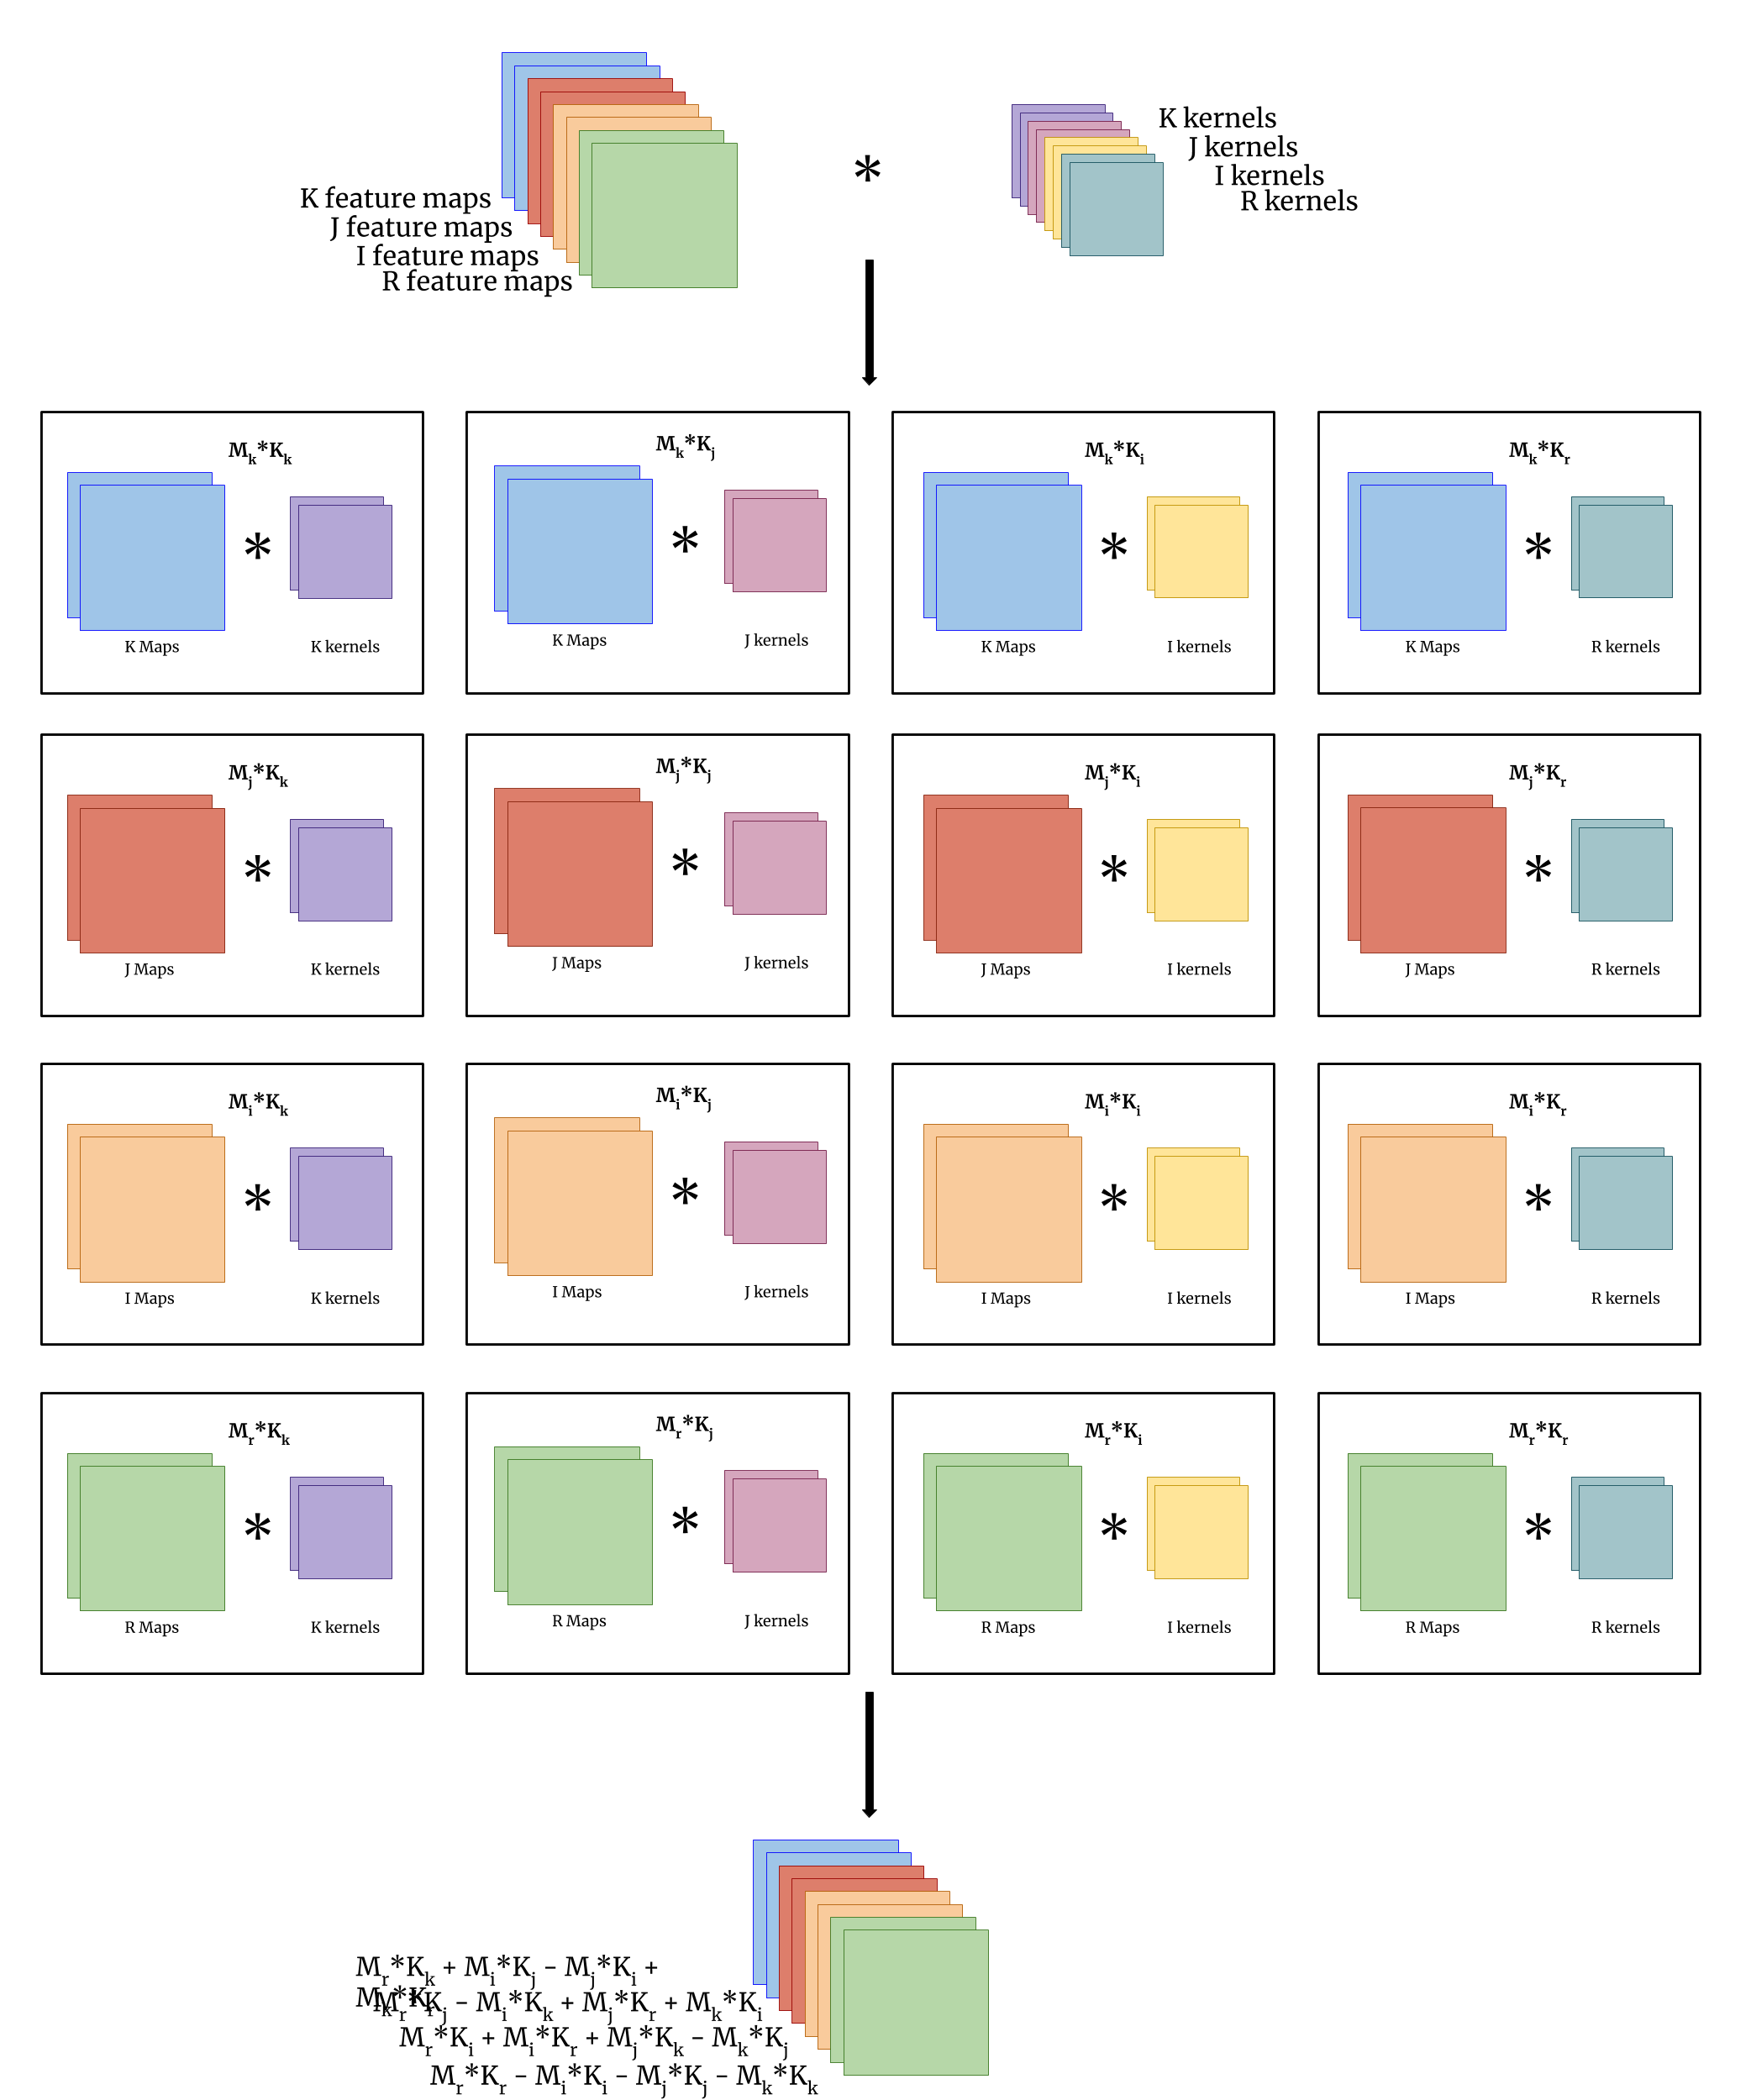
\includegraphics[width=1.0\textwidth]{figures/quatconv.png}
	\caption{An illustration of quaternion convolution.}
	\label{f:quatconv}
\end{figure*}


\subsection{Quaternion Batch-Normalization}
Batch-normalization \cite{ioffe2015batch} is used by the vast majority of all deep networks to stabilize and speed up training.
It works by keeping the activations of the network at zero mean and unit variance.
The original formulation of batch-normalization only works for real-values. 
Applying batch normalization to complex or hyper-complex numbers is more difficult, one can not simply translate and scale them such that their mean is 0 and their variance is 1.
This would not give equal variance in the multiple components of a complex or hyper-complex number.
To overcome this for complex numbers a whitening approach is used \cite{trabelsi2017deep}, which scales the data by the square root of their variances along each of the two principle components.
We use the same approach, but must whiten 4D vectors.

However, an issue arises in that there is no nice way to calculate the inverse square root of a 4~x~4 matrix.
It turns out that the square root is not necessary and we can instead use the Cholesky decomposition on our covariance matrix.
The details of why this works for whitening given in the Appendix section \ref{a:whitening}.
Now our whitening is accomplished by multiplying the \textbf{0}-centered data ($\textbf{x} - \mathbb{E}[\textbf{x}]$) by \textbf{W}:
\begin{equation}
\tilde{x} = \textbf{W}(\textbf{x} - \mathbb{E}[\textbf{x}])
\label{eq:white4d}
\end{equation}
where \textbf{W} is one of the matrices from the Cholesky decomposition of $\textbf{V}^{-1}$ where \textbf{V} is the covariance matrix given by:
\begin{align*}
\textbf{V}
=&
\begin{bmatrix}
 V_{rr} & V_{ri} & V_{rj} & V_{rk} \\
 V_{ir} & V_{ii} & V_{ij} & V_{ik} \\
 V_{jr} & V_{ji} & V_{jj} & V_{jk} \\
 V_{kr} & V_{ki} & V_{kj} & V_{kk}
\end{bmatrix} \nonumber \\
&=\left[ 
\begin{matrix*}[l]
\mbox{C}(\mathscr{R}\{\textbf{x}\}, \mathscr{R}\{\textbf{x}\}) \\
\mbox{C}(\mathscr{I}\{\textbf{x}\}, \mathscr{R}\{\textbf{x}\}) \\
\mbox{C}(\mathscr{J}\{\textbf{x}\}, \mathscr{R}\{\textbf{x}\}) \\
\mbox{C}(\mathscr{K}\{\textbf{x}\}, \mathscr{R}\{\textbf{x}\}) \\
\end{matrix*} \right. \nonumber 
\begin{matrix*}[l]
\mbox{C}(\mathscr{R}\{\textbf{x}\}, \mathscr{I}\{\textbf{x}\}) \\
\mbox{C}(\mathscr{I}\{\textbf{x}\}, \mathscr{I}\{\textbf{x}\}) \\
\mbox{C}(\mathscr{J}\{\textbf{x}\}, \mathscr{I}\{\textbf{x}\}) \\
\mbox{C}(\mathscr{K}\{\textbf{x}\}, \mathscr{I}\{\textbf{x}\}) \\
\end{matrix*} \nonumber 
\begin{matrix*}[l]
\mbox{C}(\mathscr{R}\{\textbf{x}\}, \mathscr{J}\{\textbf{x}\}) \\
\mbox{C}(\mathscr{I}\{\textbf{x}\}, \mathscr{J}\{\textbf{x}\}) \\
\mbox{C}(\mathscr{J}\{\textbf{x}\}, \mathscr{J}\{\textbf{x}\}) \\
\mbox{C}(\mathscr{K}\{\textbf{x}\}, \mathscr{J}\{\textbf{x}\}) \\
\end{matrix*} \nonumber  \left.
\begin{matrix*}[l]
\mbox{C}(\mathscr{R}\{\textbf{x}\}, \mathscr{K}\{\textbf{x}\}) \\
\mbox{C}(\mathscr{I}\{\textbf{x}\}, \mathscr{K}\{\textbf{x}\}) \\
\mbox{C}(\mathscr{J}\{\textbf{x}\}, \mathscr{K}\{\textbf{x}\}) \\
\mbox{C}(\mathscr{K}\{\textbf{x}\}, \mathscr{K}\{\textbf{x}\}) \\
\end{matrix*}  \right]
\label{eq:V4d}
\end{align*}
where C$(\cdot)$ is the covariance and $\mathscr{R}\{x\}$, $\mathscr{I}\{x\}$, $\mathscr{J}\{x\}$, and $\mathscr{K}\{x\}$ are the real, $i$, $j$, and $k$ components of $\textbf{x}$ respectively.

Real-valued batch normalization also uses two learned parameters, $\beta$ and $\gamma$. 
Our shift parameter {\boldmath$\beta$} must shift a quaternion value so it is a quaternion value itself with real, $i$, $j$, and $k$ as learnable components. 
The scaling parameter {\boldmath$\gamma$} is a symmetric matrix of size matching $\textbf{V}$ given by:
\begin{equation}
\mathbf{\gamma}
=
\left( 
\begin{array}{cccc}
V_{rr} & V_{ri} & V_{rj} & V_{rk} \\
V_{ri} & V_{ii} & V_{ij} & V_{ik} \\
V_{rj} & V_{ij} & V_{jj} & V_{jk} \\
V_{rk} & V_{ik} & V_{jk} & V_{kk}
\end{array}
\right)
\label{eq:gamma}
\end{equation}
Because of its symmetry it has only ten learnable parameters. 
The variance of the components of input $\tilde{\textbf{x}}$ are variance 1 so the diagonal of {\boldmath$\gamma$} is initialized to $1/\sqrt{16}$ in order to obtain a modulus of 1 for the variance of the normalized value. 
The off diagonal terms of {\boldmath$\gamma$} and all components of {\boldmath$\beta$} are initialized to 0.
The quaternion batch normalization is defined as:
\begin{equation}
\mbox{BN}(\tilde{\textbf{x}}) = \mathbf{\gamma}\tilde{\textbf{x}} + \mathbf{\beta}
\label{eq:qbn}
\end{equation}


\subsection{Quaternion Weight Initialization}
The proper initialization of weights is vital to convergence of deep networks. 
In this work we derive our quaternion weight initialization using the same procedure as Glorot and Bengio \cite{glorot2010understanding} and He et al. \cite{he2015delving}.

To begin we find the variance of a quaternion weight:
\begin{align}
W = &~|W|e^{(\mbox{cos}\phi_1 \textit{i} + \mbox{cos}\phi_2 \textit{j} + \mbox{cos}\phi_3 \textit{k})\theta} \nonumber \\
= &~\mathscr{R}\{W\} + \mathscr{I}\{W\} + \mathscr{J}\{W\} + \mathscr{K}\{W\}.
\label{eq:quaternion_weight}
\end{align}
where $|W|$ is the magnitude, $\theta$ and $\phi$ are angle arguments, and $\mbox{cos}^2\phi_1 + \mbox{cos}^2\phi_2 + \mbox{cos}^2\phi_3 = 1$ \cite{turner2002}.

Variance is defined as
\begin{equation}
\mbox{Var}(W) = \mathbb{E}[|W|^2] - (\mathbb{E}[W])^2,
\label{eq:variance}
\end{equation}
but since $W$ is symmetric around 0 the term $(\mathbb{E}[W])^2$ is 0. 
We do not have a way to calculate $\mbox{Var}(W) = \mathbb{E}[|W|^2]$ so we make use of the magnitude of quaternion normal values $|W|$, which follows an independent normal distribution with four degrees of freedom (DOFs).
We can then calculate the expected value of $|W|^2$ to find our variance
\begin{equation}
\mathbb{E}[|W|^2] = \int_\infty^\infty x^2 f(x) ~dx = 4\sigma^2
\label{eq:expected}
\end{equation}
where $f(x)$ is the four DOF distribution given in the Appendix.

And since $\mbox{Var}(W) = \mathbb{E}[|W|^2]$, we now have the variance of $W$ expressed in terms of a single parameter $\sigma$:
\begin{equation}
\mbox{Var}(W) = 4\sigma^2.
\label{eq:variance_sigma}
\end{equation}

To follow the Glorot and Bengio \cite{glorot2010understanding} initialization we have $\mbox{Var}(W) = 2/(n_{in}+n_{out})$, where $n_{in}$ and $n_{out}$ are the number of input and output units respectivly. 
Setting this equal to \eqref{eq:variance_sigma} and solving for $\sigma$ gives $\sigma = 1/\sqrt{2(n_{in}+n_{out})}$.
To follow He et al. \cite{he2015delving} initialization that is specialized for rectified linear units (ReLUs) \cite{nair2010rectified}, then we have $\mbox{Var}(W) = 2/n_{in}$, which again setting equal to \eqref{eq:variance_sigma} and solving for $\sigma$ gives $\sigma = 1/\sqrt{2n_{in}}$.

As shown in \eqref{eq:quaternion_weight} the weight has components $|W|$, $\theta$, and $\phi$. 
We can initialize the magnitude $|W|$ using our four DOF distribution defined with the appropriate $\sigma$ based on which initialization scheme we are following. 
The angle components are initialized using the uniform distribution between $-\pi$ and $\pi$ where we ensure the constraint on $\phi$.


\section{Experimental Results}
Our experiments covered image classification using both the CIFAR-10 and CIFAR-100 benchmarks and image segmentation using the KITTI Road Estimation benchmark.

\subsection{Classification}
We use the same architecture as the large model in \cite{trabelsi2017deep}, which is a 110 layer Residual model similar to the one in \cite{he2016deep}.
There is one difference between the real-valued network and the ones used for both the complex and hyper-complex valued networks.
Because the datasets are all real-valued the network must learn the imaginary or quaternion components.
We use the same technique as \cite{trabelsi2017deep} where there is an additional block immediately after the input which will learn the hyper-complex components
\begin{equation*}
BN \rightarrow ReLU \rightarrow Conv \rightarrow BN \rightarrow ReLU \rightarrow Conv.
\end{equation*}

Since all datasets that we work with are real-valued,
we present a way to learn their imaginary components to let the rest of the network operate in the
complex plane. 
We learn the initial imaginary component of our input by performing the operations
present within a single real-valued residual block

This means that to maintain the same approximate parameter count the number of convolution kernels for the complex network was increased.
We however did not increase the number of convolution kernels for the quaternion trials so any increase in model performance comes from the quaternion filters and at a lower hardware budget.

The architecture consists of 3 stages of repeating residual blocks where at the end of each stage the images are downsized by strided convolutions.
Each stage also doubles the previous stage's number of convolution kernels.
The last layers are a global average pooling layer followed by a single fully connected layer with a softmax function used to classify the input as either one of the 10 classes in CIFAR-10 or one of the 100 classes in CIFAR-100.

We also followed their training procedure of using the backpropagation algorithm with Stochastic Gradient Descent with Nesterov momentum \cite{nesterov1983method} set at 0.9.
The norm of the gradients are clipped to 1 and a custom learning rate scheduler is used.
The learning scheduler is the same used in \cite{trabelsi2017deep} for a direct comparison in performance.
The learning rate is initially set to 0.01 for the first 10 epochs and then set it to 0.1 from epoch 10-100 and then cut by a factor of 10 at epochs 120 and 150.
Table~\ref{t:results1} presents our results along side the real and complex valued networks.
Our quaternion model outperforms the real and complex networks on both datasets on a smaller parameter budget.

\begin{table}[h]
	\centering
		\begin{tabular}{l c c}
			\hline
			Architecture & CIFAR-10 & CIFAR-100 \\
			\hline
			\cite{he2016deep} Real & 6.37 & - \\
			\cite{trabelsi2017deep} Complex & 5.60 & 27.09 \\
			Quaternion & \textbf{5.44} & \textbf{26.01}
		\end{tabular}
	\caption{Classification error on CIFAR-10 and CIFAR-100. Note that \cite{he2016deep} is a 110 layer residual network, \cite{trabelsi2017deep} is 118 layer complex network with the same design as the prior except with additional initial layers to extract complex mappings.}
	\label{t:results1}
\end{table}

\subsection{Segmentation}
For this experiment we used the same model as the above, but cut the number of residual blocks out of the model for memory reasons given that the KITTI data is large color images.
The 110 layer model has 10, 9, and 9 residual blocks in the 3 stages talked about above, while this model has 2, 1, and 1 and does not perform any strided convolutions.
This gives a total of 38 layers.

The last layer is a $1 \times 1$ convolution with a sigmoid output so we are getting a heatmap prediction the same size as the input.
The training procedure is also as above, but the learning rate is scheduled differently.
Here we begin at 0.01 for the first 10 epochs and then set it to 0.1 from epoch 10-50 and then cut by a factor of 10 at 100 and 150.
Table~\ref{t:results2} presents our results along side the real and complex valued networks where we used Intersection over Union (IOU) for performance measure.
Quaternion outperformed the other two by a larger margin compared to the classification tasks.

\begin{table}[h]
	\centering
		\begin{tabular}{l c c}
			\hline
			Architecture & KITTI \\
			\hline
			Real & 0.747 \\
			Complex & 0.769 \\
			Quaternion & \textbf{0.827}
		\end{tabular}
	\caption{IOU on KITTI Road Estimation benchmark.}
	\label{t:results2}
\end{table}


\section{Conclusions and Proposed Research}
We have extended upon work looking into complex valued networks by exploring quaternion values.
We presented the building blocks required to build and train deep quaternion networks and used them to test residual architectures on two common image classification benchmarks.
We show that they have competitive performance by beating both the real and complex valued networks with less parameters.

Since the entirety of the work so far has been done in supervised learning, it seems prudent to explore results in unsupervised learning compared to real and complex networks.
The proposed idea is to test quaternion values in a Deep Adversarial Gaussian Mixture Autoencoder \cite{harchaoui2017deep}.
We will compare the current results of with results of both complex and quaternion networks.
Another area to explore would be in networks designed to handle 3D data given quaternions natural expressive capapilities in this area.
PointNet \cite{qi2017pointnet} and its newer variants take in a group of 3D points and use a deep network to classify the entire cloud as a class and/or classify each point in the cloud as a class.
We will compare the latest PointNet variant with complex and quaternion value models.

The majority of work was the upfront work of creating and coding the algorithms needed for deep quaternion networks.
With that done the work to explore these last two ideas only involves pulling the authors code and replacing their real layers with complex and then quaternion layers.
Including running the experiments the amount of time would be less than 6 months.


%%%%%%%%%%%%%%%%%%%%%%%%%%%%%%%%%%%%%%%%%%%%%%%%%%%%%%%%%%%%%



%%%%%%%%%%%%%%%%%%%%%%%%%%%%%%%%%%%%%%%%%%%%%%%%%%%%%%%%%%%%%
%% BIBLIOGRAPHY AND OTHER LISTS
%%%%%%%%%%%%%%%%%%%%%%%%%%%%%%%%%%%%%%%%%%%%%%%%%%%%%%%%%%%%%
%% A small distance to the other stuff in the table of contents (toc)
\addtocontents{toc}{\protect\vspace*{\baselineskip}}

%% The Bibliography
%% ==> You need a file 'literature.bib' for this.
%% ==> You need to run BibTeX for this (Project | Properties... | Uses BibTeX)
\addcontentsline{toc}{chapter}{Bibliography} %'Bibliography' into toc
\bibliographystyle{alpha} %Style of Bibliography: plain / apalike / amsalpha / ...
\bibliography{bib} %You need a file 'bib.bib' for this.

%% The List of Figures
\clearpage
\addcontentsline{toc}{chapter}{List of Figures}
\listoffigures

%% The List of Tables
\clearpage
\addcontentsline{toc}{chapter}{List of Tables}
\listoftables


%%%%%%%%%%%%%%%%%%%%%%%%%%%%%%%%%%%%%%%%%%%%%%%%%%%%%%%%%%%%%
%% APPENDICES
%%%%%%%%%%%%%%%%%%%%%%%%%%%%%%%%%%%%%%%%%%%%%%%%%%%%%%%%%%%%%
\appendix
%\input{FileName} %You need a file 'FileName.tex' for this.


\end{document}

